% UF Sample ETD Main Document Fall 2014
% 28 October, 2016: Modified slightly by LianTze Lim (Overleaf) to compile without errors
\documentclass[12pt,final,CPage]{ufthesis}
% Preamble %

% Define Packages To be used and options %
% here you define all the packages you wish to use in your paper, the ones shown are not all necessary,
% but all have purpose and can be very useful, so leave these as default and add packages as necassary
\usepackage{graphicx}
%\usepackage[dvipdfmx]{graphicx}
\usepackage{amsmath}
\usepackage{amsthm}
\usepackage{algpseudocode}
\usepackage{tabularx}
\usepackage{url}
\usepackage[letterpaper,hmargin=1in,vmargin=1in]{geometry}
\usepackage{lscape}
\usepackage{hanging}
\usepackage{longtable}
\usepackage{amsfonts}
\usepackage{amssymb}
%\usepackage[cmss]{sfmath} % Comment this line to use Times New Roman Math Typeface
\usepackage[cmbright]{sfmath} % Comment this line to use Times New Roman Math Typeface
\usepackage{subfigure}
\usepackage{rotating}
\usepackage{calc}
\usepackage{setspace}
\usepackage{ufenumerate}
\usepackage{latexsym}
\usepackage{epsf}
\usepackage{epsfig}
\usepackage{euscript}
\usepackage[format=hang,justification=raggedright,singlelinecheck=0,labelsep=period]{caption}
%\usepackage[numbers,sort&compress]{natbib} %Use this set-up for numbered reference lists
\usepackage[authoryear]{natbib} %Use this set-up if you want an un-numbered reference list
%\usepackage{hypernat}



\usepackage[hyperfootnotes=false]{hyperref}
%\usepackage[dvipdfmx,hyperfootnotes=false]{hyperref}
%\usepackage[dvips,hyperfootnotes=false]{hyperref}
\hypersetup{colorlinks=true,linkcolor=blue,anchorcolor=blue,citecolor=blue,filecolor=blue,urlcolor=blue,bookmarksnumbered=true,pdfview=FitB} %
% % %DO NOT PLACE ANY PACKAGES AFTER THE HYPERREF SET UP


\def\UrlFont{\rmfamily} %use this line for Times New Roman
% \def\UrlFont{\sffamily} %use this line for CMSS

%\allowdisplaybreaks  % % This command allows equation arrays and similar environments
% % % to break across pages to improve text flow - use only if needed.

% Prevent figures, tables or algorithms from using a separate page or column alone
\renewcommand{\topfraction}{0.85}
\renewcommand{\textfraction}{0.1}
\renewcommand{\floatpagefraction}{0.75}

% *** Do not adjust lengths that control margins, column widths, etc. ***
% *** Do not use packages that alter fonts (such as pslatex).         ***
% There should be no need to do such things with IEEEtran.cls V1.6 and later.
% correct bad hyphenation here
%\hyphenation{op-tical net-works semi-C:\Program Files\MiKTeX 2.5\miktexconduc-tor}

%------------------------------------------%

% Extra commands or misc formatting such as page alignment or output paper-size commands

%\include{extraparameters}

%------------------------------------------%

% Set your personal and paper information
\SetFullName{Shawn David Taylor}%
\SetThesisType{Dissertation}%{Dissertation} %{Thesis}
\SetDegreeType{Doctor of Philosophy}% {Doctor of Philosophy} {Master of Science}
\SetGradMonth{December}%
\SetGradYear{2019}%
\SetDepartment{Interdisciplinary Ecology}%
\SetChair{Ethan P. White}%
%\SetCochair{John W. Carver III}%uncomment this line and enter the name of your cochair inside the braces if you have one.
%If you have a cochair there two places in the ufthesis.cls file that will need to be uncommented as well
%In the "getting personal information" section about line 630
%And the "Abstract" Section around line 556
% Type your title here in all CAPS %
\SetTitle{FORECASTING PLANT PHENOLOGY: AN ASSESSMENT OF DATA SOURCES AND ESTIMATORS, AND A FULLY AUTOMATED IMPLEMENTATION}



% Define student-specific info (self-explanatory) %
%\include{userinfo}

%------------------------------------------%

% user defined commands in order to geC:\Program Files\MiKTeX 2.5\miktexnerate new commands, macros, and redefine default commands %
% user defined commands %
% Here is where you define optional commands such as macros, new commands,
% and new environments to be used in your paper

% optional command to prevent a word from breaking across a line %
\hyphenchar\font=-1


% Commands to produce proper bullet list
\newlength{\widthOfItem}
\let\Itemize=\itemize
\let\endItemize=\enditemize
\renewenvironment{itemize}{%
	\begin{Itemize}
		\setlength{\itemsep}{0.5\baselineskip}
		\setlength{\labelwidth}{2em}
		\setlength{\listparindent}{.32in}%
		\setlength{\leftmargin}{.32in}
		\setlength{\rightmargin}{0in}
		\settowidth{\widthOfItem}{\labelitemi}
		\setlength{\labelsep}{\leftmargin-\widthOfItem}
		\renewcommand{\labelitemii}{--}
		\singlespacing}{%
	\end{Itemize}}

% shortcut for setting up inserting \prime command in mathmode to avoid errors %
\newcommand{\p}{^{\prime}}

% shortcuts for prime color text
\newcommand{\red}{\textcolor[rgb]{1.00,0.00,0.00}}
\newcommand{\green}{\textcolor[rgb]{0.00,1.00,0.00}}
\newcommand{\blue}{\textcolor[rgb]{0.00,0.00,1.00}}

% Shorcut commands for mathmatical formulas %

\newcommand{\latex}{\LaTeX 2\ensuremath{\epsilon}}

% THEOREM Environments ---------------------------------------------------
%These environments are provided as a convenience - feel free to modify if needed

\newtheorem{theorem}{Theorem}[chapter]%To link the theorem to each chapter uncomment the chapter option
\newtheorem{lemma}{Lemma}%[theorem]% To link each lemma to a theorem uncomment the theorem option
\newtheorem{corollary}{Corollary}%[theorem]% To link each corollary to a theorem uncomment the theorem option
% to link a corollary to a chapter change the theorem option to chapter
\newtheorem{definition}{Definition}%[chapter] %the same is true for both definitions and assumptions
\newtheorem{assumption}{Assumption}%[chapter] %
\newtheorem{proposition}{Proposition}[chapter]
\newtheorem{algorithm}{Algorithm}[chapter]


%These were some user commands I've run across that I thought some might want to incorporate into their work
%\newcommand{\bdm}{
 %   \begin{displaymath}}

%\newcommand{\edm}{
%    \end{displaymath}}

%\newcommand{\be}{
%    \begin{equation}}

%\newcommand{\ee}{
%    \end{equation}}

%\newcommand{\bea}{
 %   \begin{eqnarray}}

%\newcommand{\eea}{
%    \end{eqnarray}}


%-------------------------------------------------------------------------------------------------------%

% Begin Main Part of Document %

\begin{document}


 % % % % % % % % % % % % % % % % % % % % % % % % % % % % % % % % % % % % % %
 % Remember - You MUST get a .bst file that matches the Journal in your
 % field that you choose as your Reference example
 % NONE of these examples will satisfy the Graduate Editorial Office
 % if they don't match your Journal example!!!!
 % NOTE: If you use a numbered reference system and your references
 % are set in parentheses rather than brackets you need to select the
 % Natbib option "numbers sort and compress" in the packages.tex file
 % % % % % % % % % % % % % % % % % % % % % % % % % % % % % % % % % % % % % %


 %Note that the path separator is a forward slash NOT a back slash
 %Place YOUR .bst file in the bst folder and use that filename (without the .bst extension)
 % as your Bibliography Style file

%\bibliographystyle{bst/abbrv}
%\bibliographystyle{bst/abbrvnat}
%\bibliographystyle{bst/abbrvurl_uf}
%\bibliographystyle{bst/alphaurl_uf}
%\bibliographystyle{bst/apa-good}
%\bibliographystyle{bst/Chicago_Web}
\bibliographystyle{bst/ecology_web}
%\bibliographystyle{bst/IEEEtran}
%\bibliographystyle{bst/mla_web}
%\bibliographystyle{bst/mla-good}
%\bibliographystyle{bst/plainnat}
%\bibliographystyle{bst/plainurl_uf}
%\bibliographystyle{bst/Science_Web}
%\bibliographystyle{bst/uf_econ}
%\bibliographystyle{bst/uffull}
%\bibliographystyle{bst/ufinit}
%\bibliographystyle{bst/unsrtnat}
%\bibliographystyle{bst/unsrturl_uf}
%\bibliographystyle{bst/plain}
%\bibliographystyle{bst/ufinit}
%\bibliographystyle{bst/plainurl_uf}


%-----------------------------------------------------------------------%

\maketitle % % % % Creates the Title page from the information entered in userinfo.tex
\makecopyright

%------------------------------------------%

\dedication{% Add your text for the dedication here between the center tags
\addvspace{4.25in}
\begin{center}\singlespacing
I dedicate this to everyone that helped revamp this template\\
\end{center}
} % %Creates the dedication - if your dedication is more than a single line
% % % % % % % % % % % % % % % % % %you will need to reduce the vspace amount to keep the text centered verticlly
% % % % % % % % % % % % % % % % % %optional - comment or delete if you are not dedicating to anyone,

%------------------------------------------%

% Make sure to keep the text within the brackets and the output should turn out correct
\acknowledge{%
Thank you to my advisor, Ethan White, for all his help and motivation these past four years. Thanks to the members of the Weecology Lab. Thank you to my friends and family.}
 % % % %Required - There is no requirement to acknowledge a particular person
% % % % % % % % % % % % % % % % %but you must acknowledge someone (funding source, committee chair, spouse)?

%------------------------------------------%

% This file includes the file which creates the table of contents %
% This creates your table of contents, list of figures, and list of tables
% the pdfbookmark line adds the word to the bookmarks of the pdf without adding it to the TOC itself
\pdfbookmark[0]{TABLE OF CONTENTS}{tableofcontents}
\tableofcontents %
\listoftables %
%\setcounter{lofdepth}{2}
\listoffigures %

% Produced list of abbreviations or symbols %
%\printindex[keylist]{KEY TO ABBREVIATIONS}{KEY TO ABBREVIATIONS}{}
%\printindex[mathlist]{KEY TO SYMBOLS}{KEY TO SYMBOLS}{%
%The list shown below gives a brief description of the major mathematical symbols defined in this work. For each
%symbol, the page number corresponds to the place where the symbol is first used.} %
 %This file creates the Table of Contents, List of Figures, and List of Objects (if any)
% % % % % % % %delete or comment the file you want to remove

%------------------------------------------%

%%This is an optional file. A list of abbreviations is NOT even suggested.
%%Best practice is to define the item the first time it is used in the document

%%%-----------List of Symbols, Nomenclature or Abbreviation--------

%% Please note: a list of Symbols, terms, acronyms, etc. is not usually the best practice.
%% More often you should simply define an abbreviation the first time it is used.
%% If you DO need to include a list like this please notice that it must be paginated manually
%% by breaking it up into page size tables. Longtable will not wrap the definition properly if
%% it extends to a second line and a similar issue is encountered when the tabbing environment
%% is used. If you have a better way of meeting the Editorial Office requirements I'd love to hear about it.

\chapter*{LIST OF SYMBOLS, NOMENCLATURE, OR ABBREVIATIONS} \addcontentsline{toc}{chapter}{LIST OF SYMBOLS} %Start
%writing here. This is optional.
\singlespacing
\begin{tabular}{l p{5in}} %if the terms in the first column are longer than 1.4 inches reduce the number 5 appropriately
$\sum$ & Denotes the summation of a series of terms\\
\\%This adds the single space between definitions (required)
$\bigcap$ & A really big bigcap\\
\\
fractal & A geometric pattern that is repeated at ever smaller
scales to produce irregular shapes and surfaces that cannot be represented by classical
geometry. Fractals are used especially in computer modeling of irregular patterns and structures in nature.}\\
\\
polynomial & (in one variable) an expression consisting of the sum of two
or more terms each of which is the product of a constant and a
variable raised to an integral power: $ax^2 + bx + c$ is a
polynomial, where $a, b,$ and $c$ are constants and $x$ is a
variable.}\\
\\
$\sum$ & Denotes the summation of a series of terms\\
\\
$\bigcap$ & A really big bigcap\\
\\
fractal & A geometric pattern that is repeated at ever smaller
scales to produce irregular shapes and surfaces that cannot be represented by classical
geometry. Fractals are used especially in computer modeling of irregular patterns and structures in nature.}\\
\\
polynomial & (in one variable) an expression consisting of the sum of two
or more terms each of which is the product of a constant and a
variable raised to an integral power: $ax^2 + bx + c$ is a
polynomial, where $a, b,$ and $c$ are constants and $x$ is a
variable.}\\
\\
$\sum$ & Denotes the summation of a series of terms\\
\\
$\bigcap$ & A really big bigcap\\
\\
fractal & A geometric pattern that is repeated at ever smaller
scales to produce irregular shapes and surfaces that cannot be represented by classical
geometry. Fractals are used especially in computer modeling of irregular patterns and structures in nature.}\\
\\
polynomial & (in one variable) an expression consisting of the sum of two
or more terms each of which is the product of a constant and a
variable raised to an integral power: $ax^2 + bx + c$ is a
polynomial, where $a, b,$ and $c$ are constants and $x$ is a
variable.}\\

\end{tabular}

\begin{tabular}{lp{5in}}
$\sum$ & Denotes the summation of a series of terms\\
\\
$\bigcap$ & A really big bigcap\\
\\
fractal & A geometric pattern that is repeated at ever smaller
scales to produce irregular shapes and surfaces that cannot be represented by classical
geometry. Fractals are used especially in computer modeling of irregular patterns and structures in nature.}\\
\\
polynomial & (in one variable) an expression consisting of the sum of two
or more terms each of which is the product of a constant and a
variable raised to an integral power: $ax^2 + bx + c$ is a
polynomial, where $a, b,$ and $c$ are constants and $x$ is a
variable.}\\
\\
$\sum$ & Denotes the summation of a series of terms\\
\\
$\bigcap$ & A really big bigcap\\
\\
fractal & A geometric pattern that is repeated at ever smaller
scales to produce irregular shapes and surfaces that cannot be represented by classical
geometry. Fractals are used especially in computer modeling of irregular patterns and structures in nature.}\\
\\
polynomial & (in one variable) an expression consisting of the sum of two
or more terms each of which is the product of a constant and a
variable raised to an integral power: $ax^2 + bx + c$ is a
polynomial, where $a, b,$ and $c$ are constants and $x$ is a
variable.}\\
\\
$\sum$ & Denotes the summation of a series of terms\\
\\
$\bigcap$ & A really big bigcap\\
\\
fractal & A geometric pattern that is repeated at ever smaller
scales to produce irregular shapes and surfaces that cannot be represented by classical
geometry. Fractals are used especially in computer modeling of irregular patterns and structures in nature.}\\
\\
polynomial & (in one variable) an expression consisting of the sum of two
or more terms each of which is the product of a constant and a
variable raised to an integral power: $ax^2 + bx + c$ is a
polynomial, where $a, b,$ and $c$ are constants and $x$ is a
variable.}\\
\\
\end{tabular}
\doublespacing




%------------------------------------------%
% This line adds the word CHAPTER to the TOC just before the listing of the chapter and subsections begins
\addtocontents{toc}{\protect\addvspace{10pt}\noindent{CHAPTER}\protect\hfill\par}{}% This extra line adds the word CHAPTER to the table of contents %
\phantomsection
% Write in only the text of your abstract, all the extra heading jargon is automatically taken care of
\begin{abstract}
Despite phenology being an integral part of ecological systems there is currently no near-term plant phenology forecast due to several challenges. Phenological data at an adequate scale in North America is from volunteer citizen science programs, and due to potentially observer bias may not be suitable for driving predictive models. These data are also status-based, in that they do not indicate transition dates directly, such as the timing of flowering and leaf out, but instead indicate the presence or absence of these phenophases. Implementing a forecast system also has numerous computational challenges, such as managing models for numerous species, ingesting large-scale climate forecasts, and disseminating those forecasts in a reliable and interpretable way. This dissertation addresses three questions. First we compared citizen science phenological data with data from long-term research studies. We found that models built with these different data sets resulted in different parameters, potentially resulting in conflicting inferences. Yet models from the two data sources produced similar estimates for phenological events, suggesting the large-scale citizen science data are suitable for predictive modeling. Second, we used a 10 year dataset of near daily phenological observations to test different methods of estimating transition dates. The best estimator depended on the scale of the data, with a method derived from a Weibull distribution being the best for a population of plants, while a method using the first observed date of a phenophase, combined with the most recent absence, was the best for individual plants. Finally, we implemented an automated plant phenology forecast system which predicts the timing of budburst, flowers, ripe fruit, and fall colors for 77 species across the United States up to 6 months in advance. We describe the key steps in the pipeline, including: 1) fitting phenology models, 2) acquiring climate data; 3) making predictions for phenological events; 4) disseminating those predictions; and 5) fully automating the pipeline. From the lessons learned we provide guidance in developing large-scale near-term ecological forecast systems more generally and to help advance the use of automated forecasting in ecology. 
\end{abstract}
 %The abstract is created using this file and userinfo.tex
% % % % % % % % % % %If you have a c-chair you must uncomment that line in userinfo.tex AND find the
% % % % % % % % % % %co-chair lines in ufthesis.cls and un-comment those as well

%-----------------------------------------------------------------------%

% This section encompasses the main body of the paper from all the content through to the biographical sketch

% Chapters to be included (more can be added by creating a new chapter#.tex %
% file and then implementing the \inlcude{chapter#.tex} command as seen below %
\chapter{INTRODUCTION} \label{intro}

We don't make the Chapter titles in All Caps Automatically because it is easier for you to type your Chapter Titles in uppercase than for those that need to have mixed case in their titles to find the correct command in the ufthesis.cls file and change it there. \cite{strickler1998contamination}

\section{The Section Command Text Should Be in Title Case}

 Title case is where all principal words are capitalized except prepositions, articles, and conjunctions.  \cite{green2008wrinkle}

\subsection{Subsection Commands Are Also in Title Case}
The difference, of course, are the second level headings are left-aligned

\subsubsection{Subsubsections are in sentence case}
The third level subheadings are left-aligned but in sentence case. Only the first letter and any proper nouns are capitalized.

\subsubsection{If you divide a section, you must divide it into two, or more, parts}

{\bf Paragraph headings.} There is no official fourth level heading. Do not use the Paragraph heading feature in LaTeX, simply apply the bold characteristic to the first few words of a paragraph followed by a colon or period.

\subsection{I Need Another Second Level Heading in This Section}

Aliquam mi nisi, tristique at rhoncus quis, consectetur non mi. Phasellus blandit quam ligula, a viverra lacus commodo at. In iaculis nisl vel pretium sollicitudin. In efficitur massa vel elit sollicitudin, vel auctor sapien cursus. Proin feugiat sapien a mi tempus, in consequat augue cursus. Nulla sed sagittis purus. Nunc eu consequat orci, eu laoreet enim. Ut euismod tincidunt sem, eget lacinia dui luctus eu. Aliquam mi augue, faucibus id semper vitae, porta ac ligula. Morbi sed ultrices odio. Mauris id luctus ex. Nulla ac libero dictum, interdum turpis lacinia, scelerisque leo. Praesent varius orci ac eros varius pharetra.

\section{Image Handling in XeLaTeX}

One of the biggest reasons for switching from the dvipdfm/dvipdfmx methods of compiling is the improved image handling capabilities. EPS, Bit-mapped, PDF, JPG, and PNG formats work well with the xelatex process.

\subsection{The Traditional EPS Format}

EPS format is the traditional format for LaTeX, but EPS files can be very large and many programs can't create or view these images. There are many programs that are used to interpret data and output the results as an EPS format image. It has been my experience that there are bounding box problems with these figures. On many occasions we have opened the image in Adobe Photoshop and, without making any changes, saved the document as a Photoshop EPS file, re-compiled the document, and the image worked correctly, so if you are having problems with an EPS image not showing in your document correctly, try this fix first.


\begin{figure}[htbp]
  \centering
    \includegraphics[width=5in]{images/diagram}
    \caption[EPS format diagram. Note: no filetype is designated by adding an extension.]{EPS format diagram. Note: no filetype is designated by adding an extension. The file type is determined and the correct procedure is automatically chosen by xelatex.}
\end{figure}


Quisque malesuada a leo eget ullamcorper. Curabitur ut aliquam quam. Nam quis quam id mauris aliquam blandit porttitor sit amet quam. Donec ut erat eleifend turpis finibus pulvinar.

\subsection{Bitmapped Images Work As Well}

Bitmapped images are a standard file type on PCs, but these files are also usually very large so compressed images may be a better alternative.

\begin{figure}[htbp]
  \centering
    \includegraphics[width=5in]{images/eagle}
    \caption[BMP format drawing. Note: no filetype is designated by adding an extension.]{BMP format drawing. Note: no filetype is designated by adding an extension. The file type is determined and the correct procedure is automatically chosen by xelatex.}
\end{figure}

Morbi hendrerit risus nec quam posuere viverra. Donec quis tellus faucibus, molestie arcu sed, congue urna. Duis eget neque ac libero pulvinar porta eget et magna. Donec a magna eu eros suscipit cursus ac vitae nisl. Vivamus ligula purus, congue sed tortor blandit, ultrices egestas nisl.

\subsection{Not to Mention PDF}

It is often very handy to be able to include a pdf file as an image. By using XeLaTeX this is usually just matter of setting the size, or scale properties correctly.

\begin{figure}[htbp]
  \centering
    \includegraphics[scale=1.0]{images/graph.pdf}
    \caption[PDF format graph. Note: no filetype is designated by adding an extension.]{PDF format graph. Note: no filetype is designated by adding an extension. The file type is determined and the correct procedure is automatically chosen by xelatex.}
\end{figure}

Nulla mattis augue lacus. Nam non lectus dolor. Cras ac quam vel justo elementum vestibulum. Integer vulputate pulvinar lacus sit amet pulvinar.

\subsection{JPG Is Absolutely Necessary}

For photographs, JPG is the most common format. This format is a fraction of the size of Bit-mapped images and can deliver very good quality at a much smaller overhead. Vestibulum eu lectus vel orci dictum vehicula. Proin id maximus dolor. Integer augue ante, pulvinar ac erat vitae, porttitor ullamcorper libero. \cite{l2012wrinkle}

\begin{figure}[htbp]
  \centering
    \includegraphics[width=5in]{images/nebula}
    \caption[JPG format image. Note: no filetype is designated by adding an extension.]{JPG format image. Note: no filetype is designated by adding an extension. The file type is determined and the correct procedure is automatically chosen by xelatex.}
\end{figure}

Nunc blandit scelerisque velit, ac facilisis dui finibus et. Sed facilisis tortor vel commodo luctus. Donec est felis, malesuada id nibh in, accumsan malesuada lectus. Sed lobortis volutpat felis, vitae aliquet augue congue id. Fusce ut odio tincidunt, condimentum nulla vel, pharetra arcu.

\subsection{PNGs Will Help Make Files Smaller}

PNG files are even smaller than JPGs and are very good when text and images are combined.

\begin{figure}[htbp]
  \centering
    \includegraphics[width=5in]{images/theworld}
    \caption[PNG format map. Note: no filetype is designated by adding an extension.]{PNG format map. Note: no filetype is designated by adding an extension. The file type is determined and the correct procedure is automatically chosen by xelatex.}
\end{figure}



Aenean condimentum libero sed mi porta, tempus ullamcorper lectus venenatis. Aliquam in diam dolor. Maecenas tempus consectetur sem et pulvinar. Aenean aliquam at metus ut hendrerit. Vivamus molestie ac neque eu luctus. Nam convallis maximus quam non lobortis. Fusce sit amet lorem et massa convallis aliquet at sit amet nulla. Suspendisse nec ex elit. Aenean gravida, sapien vitae congue commodo, urna turpis ornare libero, at cursus risus libero in erat. \cite{Rust94}

\section{GIF, TIF, and Others}

Other file formats have not been successful, with or without file extensions. The tests have not been exhaustive so if you have a different type, give it a try. GIF, and TIF both do NOT work at this time.

Aliquam mi nisi, tristique at rhoncus quis, consectetur non mi. Phasellus blandit quam ligula, a viverra lacus commodo at. In iaculis nisl vel pretium sollicitudin. In efficitur massa vel elit sollicitudin, vel auctor sapien cursus. Proin feugiat sapien a mi tempus, in consequat augue cursus. Nulla sed sagittis purus. Nunc eu consequat orci, eu laoreet enim. Ut euismod tincidunt sem, eget lacinia dui luctus eu. Aliquam mi augue, faucibus id semper vitae, porta ac ligula. Morbi sed ultrices odio. Mauris id luctus ex. Nulla ac libero dictum, interdum turpis lacinia, scelerisque leo. Praesent varius orci ac eros varius pharetra.



Nunc blandit scelerisque velit, ac facilisis dui finibus et. Sed facilisis tortor vel commodo luctus. Donec est felis, malesuada id nibh in, accumsan malesuada lectus.
\begin{itemize} %
    \item WinEDT: This text editor is recommended for use editing \TeX-files as it has many useful built in macros and is easy to use  %
    \item This program can be found and downloaded here: \url{http://www.winedt.com/} %
    \item The GIMP (GNU Image Manipulation Program) %
    \begin{itemize}%
        \item A freeware graphics editing program for picture editing and file conversions %\vspace{-12pt}%
        \item Comparable to Adobe Photoshop %\vspace{-12pt}%
        \item Can be downloaded here: \url{http://www.gimp.org/}%
    \end{itemize}
    \item A good reference of \LaTeX 2\ensuremath{\epsilon} commands%
    \begin{itemize}
        \item This should be included on the ETD website here: \url{http://etd.helpdesk.ufl.edu/tex.php}
    \end{itemize}
\end{itemize} %


Sed lobortis volutpat felis, vitae aliquet augue congue id. Fusce ut odio tincidunt, condimentum nulla vel, pharetra arcu. In ultricies libero diam, nec rutrum magna vehicula nec. Praesent dictum eros sit amet turpis ultricies, eleifend condimentum dui imperdiet. Donec congue urna ante, id rutrum mi commodo a. Vivamus id tincidunt nunc. Morbi id lacus ut augue ultricies convallis. Duis a lectus quis ante pretium scelerisque nec nec nisi. In id porta justo, at euismod diam. Suspendisse vel tempus arcu. Praesent vel cursus nisi, ac rhoncus odio.


\chapter{LITERATURE REVIEW} \label{lit}

\section{Dolor Sit Amet}

 Many of the problems in theses and dissertations involve tables. The UF Graduate Counsel is very specific in the Table Requirements. There should be no vertical lines in tables and only three horizontal lines. No bold text, etc., see the web site for the complete list of requirements. One simple improvement can be incorporated by using tabularx instead of the tabular environment. This allows a table to be stretched the full text width easily, which avoids the centered or left aligned issue. Table \ref{first} is an examble of the tabularx code. Consectetur adipiscing elit. Fusce eget tempus lectus, non porttitor tellus. Aliquam molestie sed urna quis convallis. Aenean nibh eros, aliquam non eros in, tempus lacinia justo. In magna sapien, blandit a faucibus ac, scelerisque nec purus.
 
 \begin{table}[htbp]
    \caption{A sample Table}\label{first}
    \begin{tabularx}{6.5in}{XXX}
      \hline
      First & Second & Third \\
      \hline
      12 & 45 & 26 \\
      17 & 32 & 93 \\
      text & 51 & can be there too. \\	
      \epsfig{figure=images/cat.eps, scale=1} & 28 & Figures too - a cat. \\
      \begin{turn}{0}\epsfig{figure=images/mouse.eps, scale=0.25}\end{turn} & 000 & and a mouse! \\
      \hline
    \end{tabularx}
\end{table}
 
 
 Praesent fermentum felis nec massa interdum, vel dapibus mi luctus. Cras id fringilla mauris. Ut molestie eros mi, ut hendrerit nulla tempor et. Pellentesque tortor quam, mattis a scelerisque nec, euismod et odio. Mauris rhoncus metus sit amet risus mattis, eu mattis sem interdum.

\subsection{Platea Dictumst}
Donec convallis scelerisque ante, in sollicitudin orci laoreet eu. Nam arcu magna, semper vel lorem eu, venenatis ultrices est. Nam aliquet ut erat ac scelerisque. Maecenas ut molestie mi. Phasellus ipsum magna, sollicitudin eu ipsum quis, imperdiet cursus turpis. Etiam pretium enim a fermentum accumsan. Morbi vel vehicula enim.


\subsection{Long (and/or Wide) Tables}

Another problem in LaTeX is the inability to handle long tables. While there are some packages that address this problem none of them quite fit the Editorial Office guidelines. The caption is not repeated but we do need "Table x-y. Continued" on each subsequent page and a repeat of the column headings on each page as well. The following table is the best example of the correct format I can produce. The disadvantage of this method is that much of it is manually set up and changes in the text will cause changes in the table. \citep{Moffatt69} For best results avoid the use of footnotemark and footnotetext commands inside of tables and try to keep your footnotes outside of floats whenever possible.



\begin{table}
\caption{Feasible triples for highly variable Grid, MLMMH.} \label{tbl1}
\begin{tabularx}{6.5 in}{r l X}
\hline {{Time (s)}} & {{Triple chosen}} & {{Other feasible triples}} \\ \hline
0 & (1, 11, 13725) & (1, 12, 10980), (1, 13, 8235), (2, 2, 0), (3, 1, 0) \\
2745 & (1, 12, 10980) & (1, 13, 8235), (2, 2, 0), (2, 3, 0), (3, 1, 0) \\
5490 & (1, 12, 13725) & (2, 2, 2745), (2, 3, 0), (3, 1, 0) \\
8235 & (1, 12, 16470) & (1, 13, 13725), (2, 2, 2745), (2, 3, 0), (3, 1, 0) \\
10980 & (1, 12, 16470) & (1, 13, 13725), (2, 2, 2745), (2, 3, 0), (3, 1, 0) \\
13725 & (1, 12, 16470) & (1, 13, 13725), (2, 2, 2745), (2, 3, 0), (3, 1, 0) \\
16470 & (1, 13, 16470) & (2, 2, 2745), (2, 3, 0), (3, 1, 0) \\
19215 & (1, 12, 16470) & (1, 13, 13725), (2, 2, 2745), (2, 3, 0), (3, 1, 0) \\
21960 & (1, 12, 16470) & (1, 13, 13725), (2, 2, 2745), (2, 3, 0), (3, 1, 0) \\
24705 & (1, 12, 16470) & (1, 13, 13725), (2, 2, 2745), (2, 3, 0), (3, 1, 0) \\
27450 & (1, 12, 16470) & (1, 13, 13725), (2, 2, 2745), (2, 3, 0), (3, 1, 0) \\
30195 & (2, 2, 2745) & (2, 3, 0), (3, 1, 0) \\
32940 & (1, 13, 16470) & (2, 2, 2745), (2, 3, 0), (3, 1, 0) \\
35685 & (1, 13, 13725) & (2, 2, 2745), (2, 3, 0), (3, 1, 0) \\
38430 & (1, 13, 10980) & (2, 2, 2745), (2, 3, 0), (3, 1, 0) \\
41175 & (1, 12, 13725) & (1, 13, 10980), (2, 2, 2745), (2, 3, 0), (3, 1, 0) \\
43920 & (1, 13, 10980) & (2, 2, 2745), (2, 3, 0), (3, 1, 0) \\
46665 & (2, 2, 2745) & (2, 3, 0), (3, 1, 0) \\
49410 & (2, 2, 2745) & (2, 3, 0), (3, 1, 0) \\
52155 & (1, 12, 16470) & (1, 13, 13725), (2, 2, 2745), (2, 3, 0), (3, 1, 0) \\
54900 & (1, 13, 13725) & (2, 2, 2745), (2, 3, 0), (3, 1, 0) \\
57645 & (1, 13, 13725) & (2, 2, 2745), (2, 3, 0), (3, 1, 0) \\
60390 & (1, 12, 13725) & (2, 2, 2745), (2, 3, 0), (3, 1, 0) \\
63135 & (1, 13, 16470) & (2, 2, 2745), (2, 3, 0), (3, 1, 0) \\
65880 & (1, 13, 16470) & (2, 2, 2745), (2, 3, 0), (3, 1, 0) \\
68625 & (2, 2, 2745) & (2, 3, 0), (3, 1, 0) \\
71370 & (1, 13, 13725) & (2, 2, 2745), (2, 3, 0), (3, 1, 0) \\
74115 & (1, 12, 13725) & (2, 2, 2745), (2, 3, 0), (3, 1, 0) \\
76860 & (1, 13, 13725) & (2, 2, 2745), (2, 3, 0), (3, 1, 0) \\
79605 & (1, 13, 13725) & (2, 2, 2745), (2, 3, 0), (3, 1, 0) \\
82350 & (1, 12, 13725) & (2, 2, 2745), (2, 3, 0), (3, 1, 0) \\
85095 & (1, 12, 13725) & (1, 13, 10980), (2, 2, 2745), (2, 3, 0), (3, 1, 0) \\
87840 & (1, 13, 16470) & (2, 2, 2745), (2, 3, 0), (3, 1, 0) \\
90585 & (1, 13, 16470) & (2, 2, 2745), (2, 3, 0), (3, 1, 0) \\
93330 & (1, 13, 13725) & (2, 2, 2745), (2, 3, 0), (3, 1, 0) \\
96075 & (1, 13, 16470) & (2, 2, 2745), (2, 3, 0), (3, 1, 0) \\
98820 & (1, 13, 16470) & (2, 2, 2745), (2, 3, 0), (3, 1, 0) \\
101565 & (1, 13, 13725) & (2, 2, 2745), (2, 3, 0), (3, 1, 0) \\
104310 & (1, 13, 16470) & (2, 2, 2745), (2, 3, 0), (3, 1, 0) \\
107055 & (1, 13, 13725) & (2, 2, 2745), (2, 3, 0), (3, 1, 0) \\
109800 & (1, 13, 13725) & (2, 2, 2745), (2, 3, 0), (3, 1, 0) \\
112545 & (1, 12, 16470) & (1, 13, 13725), (2, 2, 2745), (2, 3, 0), (3, 1, 0) \\
\hline
\end{tabularx}
\end{table}

\begin{table}[h!t!]
\begin{tabularx}{6.5 in}{r l X}
\multicolumn{3}{l}{Table \ref{tbl1}. Continued}\\%
\hline {{Time (s)}} & {{Triple chosen}} & {{Other feasible triples}} \\ \hline
115290 & (1, 13, 16470) & (2, 2, 2745), (2, 3, 0), (3, 1, 0) \\
118035 & (1, 13, 13725) & (2, 2, 2745), (2, 3, 0), (3, 1, 0) \\
120780 & (1, 13, 16470) & (2, 2, 2745), (2, 3, 0), (3, 1, 0) \\
123525 & (1, 13, 13725) & (2, 2, 2745), (2, 3, 0), (3, 1, 0) \\
126270 & (1, 12, 16470) & (1, 13, 13725), (2, 2, 2745), (2, 3, 0), (3, 1, 0) \\
129015 & (2, 2, 2745) & (2, 3, 0), (3, 1, 0) \\
131760 & (2, 2, 2745) & (2, 3, 0), (3, 1, 0) \\
134505 & (1, 13, 16470) & (2, 2, 2745), (2, 3, 0), (3, 1, 0) \\
137250 & (1, 13, 13725) & (2, 2, 2745), (2, 3, 0), (3, 1, 0) \\
139995 & (2, 2, 2745) & (2, 3, 0), (3, 1, 0) \\
142740 & (2, 2, 2745) & (2, 3, 0), (3, 1, 0) \\
145485 & (1, 12, 16470) & (1, 13, 13725), (2, 2, 2745), (2, 3, 0), (3, 1, 0)\\%
148230 & (2, 2, 2745) & (2, 3, 0), (3, 1, 0) \\
150975 & (1, 13, 16470) & (2, 2, 2745), (2, 3, 0), (3, 1, 0) \\
153720 & (1, 12, 13725) & (2, 2, 2745), (2, 3, 0), (3, 1, 0) \\
156465 & (1, 13, 13725) & (2, 2, 2745), (2, 3, 0), (3, 1, 0) \\
159210 & (1, 13, 13725) & (2, 2, 2745), (2, 3, 0), (3, 1, 0) \\
161955 & (1, 13, 16470) & (2, 2, 2745), (2, 3, 0), (3, 1, 0) \\
164700 & (1, 13, 13725) & (2, 2, 2745), (2, 3, 0), (3, 1, 0) \\
\hline
\end{tabularx}
\end{table}

\section{Ex id ullamcorper commodo}
Augue sapien mattis leo, nec accumsan turpis quam at neque. Ut pellentesque velit sed placerat cursus. Integer congue urna non massa dictum, a pellentesque arcu accumsan. Nulla posuere, elit accumsan eleifend elementum, ipsum massa tristique metus, in ornare neque nisl sed odio. Nullam eget elementum nisi. Duis a consectetur erat, sit amet malesuada sapien. Aliquam nec sapien et leo sagittis porttitor at ut lacus. Vivamus vulputate elit vitae libero condimentum dictum. Nulla facilisi. Quisque non nibh et massa ullamcorper iaculis.

Integer laoreet bibendum arcu non pulvinar. Curabitur ac magna nibh. Phasellus sed nisi semper, molestie neque at, tempus lacus. Aenean vitae lacinia est. Phasellus aliquam lacus sit amet placerat molestie. Sed sit amet bibendum lectus, ac ornare ligula. Curabitur porttitor interdum tortor a dignissim. Quisque a placerat nibh. Phasellus lobortis imperdiet augue, non congue est bibendum eu. Vivamus tincidunt quam eu fringilla laoreet.

Maecenas efficitur dolor et ipsum convallis, ut fringilla neque luctus. Donec ac nisl quis leo gravida accumsan sit amet sed tellus. Quisque placerat hendrerit augue sit amet aliquet. Vestibulum laoreet consequat nunc, et egestas nisl auctor et. Duis scelerisque vulputate placerat. Proin tempus ligula ac tempor eleifend. Nullam est odio, commodo quis nisl eu, feugiat efficitur purus.

Duis egestas in mauris vel efficitur. Sed a faucibus sem, non euismod enim. Maecenas nec nulla justo. Suspendisse ut orci ac mi aliquet tincidunt ac eget quam. Quisque ac mi sagittis, dapibus dui a, facilisis neque. Aenean euismod orci sem, non imperdiet ipsum pulvinar ac. Proin eu vestibulum magna, eu ullamcorper nulla. Etiam enim felis, dignissim eget commodo ac, faucibus nec justo. Nulla condimentum velit imperdiet ligula aliquam semper. Nulla facilisi. Ut in lobortis metus, at dictum ipsum. Suspendisse facilisis nec eros eget mollis. Vestibulum eget dolor ac mauris lobortis gravida. Suspendisse consectetur orci in risus pharetra, sed eleifend nisl lacinia. Mauris augue nibh, commodo sed sem at, congue molestie massa. Suspendisse sodales aliquet tellus, a tristique nunc aliquam id.


\chapter{ESTIMATING TRANSITION DATES FROM STATUS-BASED PHENOLOGICAL OBSERVATIONS: A TEST OF METHODS}

\section{Background}
Most phenological datasets use status-based monitoring, where over time observers record the current state of a single plant (ie. leaves present or absent) regardless of recent or impending transitions. This includes research using herbarium records, where the presence or absence of flowers and other phenophases is inferred from their presence on a specimen \citep{willis2017}. To make use of status-based data in most phenological models the transition date must first be estimated, and there are several methods available. Here I compared the most common estimators using dataset of intensely sampling phenological observations. \renewcommand*{\thefootnote}{}\footnote{Reprinted with permission from Taylor, S.D. 2019. Estimating flowering transition dates from status-based phenological observations: a test of methods. PeerJ 7:e7720 https://doi.org/10.7717/peerj.7720}

Two of the most common estimators are the first observed and mean occurrence day methods, where either the first observation in a year or the mean dates for all observations within a year is used as an estimate for a phenophase transition and peak dates, respectively \citep{willis2017}. The first observed method has been shown to be biased in several instances, while the mean occurrence date is considered a reliable estimator for the midpoint or peak of a phenophase \citep{miller-rushing2008, moussus2010, bertin2015}. Recently more robust methods have been introduced. \cite{templ2017} used survival modelling to estimate the median date of flowering and \cite{pearse2017} used an extinction model to estimate the first flowering date. Using repeated observations of individual plants, as opposed to observations from across a population, site, or region, allows for more reliable estimates. For example if flowers are not present during one visit but present during the next, the transition of flowers opening is constrained to the window between the two visits \citep{gerst2016}. Studies of bird migration phenology face similar challenges and several estimators have been used to model the first arrival dates. Examples include logistic regression \citep{mayor2017} and General Additive Models (GAMs) \citep{moussus2009, newson2016, linden2017}. To date no comparison has been made of these different transition date estimators for plant phenology. 

Furthermore, there are no clear guidelines for using estimators across different spatial scales. Over a latitudinal gradient the transition of a phenophase for a single species can last several weeks to months, and even at the local scale can vary due to many factors \citep{diez2012, zhang2017}. Studies which estimate transition dates have combined observations from individual plants \citep{gerst2016, taylor2019}, sites or populations of plants \citep{schaber2002, linkosalo2008, basler2016}, or entire regions \citep{calinger2013, park2014}. How different phenological estimators perform across spatial scales is currently unknown. 

A comparison of estimators is difficult since, due to infrequent sampling, the true date of transitions is rarely known. Previously \cite{moussus2010} used simulated data to test the ability of different estimators to detect shifts in phenological distributions. Here I expand on this prior study by using a dataset of flowering observations where, due to the unique physiology of the focal species, transition dates can be calculated with high precision, and the efficacy of the different estimators directly compared. To determine how these estimators perform using different sources of phenological data, such as those from herbarium records or crowd-source applications, I performed this analysis across two different scales (population and individual level transition dates), with varying sample sizes, and with varying proportions of observed flowering presence.

\section{Methods}

\subsection{Phenological Data}

I used phenological observations of the perennial forb \textit{Echinacea angustifolia} collected in Minnesota, U.S.A. in the years 1995-2015 \citep{waananen2018a, waananen2018b} to test the accuracy of different transition date estimators. The data consist of the start and end date of flowering (defined as the start and end of pollen production) for 286 individual plants in a 0.5 ha plot from the 11 years of sampling, where the sampling frequency was at least every 3 days during pollen production. The flowering of \textit{E. angustifolia} is such that the true start date of flowering can be inferred very precisely for an individual plant. The flowering heads of \textit{E. angustifolia} consist of 80-250 disk flowers in several rows. The bottom most row flowers first, with each adjacent row flowering every day afterwards. This pattern was used to determine the date of first flowering for an individual to within 2 days for flowering onset and 3 days for flowering end \citep{wagenius2004, waananen2018a}. With this information a true start and end date of flowering for the entire population can be approximated.

Different interpretations of phenological metrics can yield different results \citep{renzi2019}, thus with the \textit{E. angustifolia} dataset I used strict definitions in calculating the true values used in the analysis. For each year I calculated the following population-level metrics: 1) the start of flowering as defined by the day of year (DOY) of the first observed flower, 2) peak flower defined as the DOY when the most flowers were observed in a given year, 3) the end of flowering as defined by the last DOY a flower was observed. I also calculated two individual level metrics: 1) the start and 2) end DOY of flowering for each individual plant in each year.

To simulate status-based data of a plant population I first determined the flowering status (either present or absent) for every individual plant on every DOY 1-365, then randomly sampled from these dates. Thus an observation could be of flowers present or absent. Flowering absence observations are possible throughout the year as no individual flowers for the full duration of the season. I performed a Monte Carlo analysis, where for every year I repeated this 1000 times with varying sample sizes (10, 50, and 100 observations) and varying levels of flowering presence being observed (25\%, 50\%, and 75\%). For example, with flowering presence set to 25\% using 100 observations only 25 observations were allowed to be of flower presence while the rest were of flower absence, all being randomly chosen from the full calendar year. The variation in sample size and ratio of flowering presence observations simulate patterns seen in non-systematic phenological datasets, such as the those from herbarium records or volunteer contributions. These patterns stem from biases in the time of year of sampling, infrequent or sporadic sampling, or variations in observer effort \citep{dickinson2010, willis2017, daru2018}. 

For individual level flowering estimates I performed the same random sampling routine for every individual in every year using sample sizes of 5, 10, and 20 observations, and flowering presence ratios of 25\%, 50\%, and 75\%. I only used individuals which were in flower for more than 20 days, since below that there would not be enough data in the lowest sample size and flowering presence classes. I repeated this 20 times for each individual in every year in the Monte Carlo analysis. 

Each estimator, described below, was fit to each random sample (Table 1). For the population estimates this resulted in 11,000 estimates for each estimator, and sample size/flowering presence combination. For the individual estimates this resulted in 4840 estimates for each estimator and sample size/flowering presence combination. Estimators were compared using the R\textsuperscript{2} value between estimated and observed dates of metrics, and by examining the density of errors from all Monte Carlo estimates.

\subsection{Estimators}

The First Observed method uses the earliest DOY of flowering as the estimate for the start of flowering. Analogous to this is the last observed DOY for estimating the end of flowering. These were used in both the population and individual level analysis.  

The Midway method uses the midway date between the first observed flowering date and the most prior observation of flowering absence for an individual plant. This can be improved by applying a restriction whereas only individuals with an observed absence within 7 days of the first observed presence are used \citep{gerst2016}. Applying this restriction reduces the final sample size available for modelling though. The Midway method was used to estimate onset and end in the individual analysis (Midway and Midway 7-Day), and in the population analysis by using the mean onset date from all individuals (Mean Midway and Mean Midway 7-Day). For all cases I noted the rate at which this could not be calculated due to inadequate sampling (ie. if no individuals have an absence observation within 7 days prior to the first presence, than no estimate can be made). 

The Weibull method fits a Weibull distribution to only the flowering presence observations, thus is advantageous when no absence observations are available. The flexible Weibull distribution can model a variety of shapes, and is commonly used to used to estimate the start or end of a process. The estimated date of first flowering is the sum of the dates of all flowering weighted by the joint Weibull distribution and is equivalent to estimating an extinction date \citep{roberts2003, pearse2017}. This was used for both population and individual level estimates. Code for this in the R language was obtained from \cite{pearse2017} and is provided in the code repository. 

The Logistic method fits a generalized linear model to both presence and absence observations using a binomial distribution, where the DOY was used to explain the presence or absence of flowering. Prior to fitting all flowering absence observations after the last observed flowering presence were excluded. The expected probability of observing a flower was calculated for all DOYs 1-365, and the estimated onset of flowering was the first DOY in the season in which the expected probability exceeded a given threshold. The inverse of this is used to estimate the end of flowering. All absence observations prior to the first observed flowering date were excluded, the expected probability was calculated for all DOYs 1-365, and the first DOY where the probability of flowering falls below the threshold was the estimate for the end of flowering. I evaluated a range of probability thresholds (0.05, 0.25, 0.50 ,0.75, and 0.95) and used the one with the highest R\textsuperscript{2} for each combination of metric, sample size, and flowering presence ratio. This method was used in both the population and individual level analysis. 

The GAM method is unique in that it can potentially estimate the full flowering phenology for a season (onset, peak, and end) using smoothing splines. Similar to the Logistic method, a general additive model was fit with a binomial distribution and DOY explaining the presence or absence of flowers, where the DOY was a thin plate regression spline. The expected probability of flowering was calculated for all DOYs 1-365. The estimated onset date was the first DOY in which the probability exceeded a given threshold. The estimated peak flowering date was the DOY with the maximum probability in a given year. The estimated end of flowering was the first DOY, after the peak, in which the probability fell below the threshold. As in the Logistic method I evaluated five probability thresholds and chose the one with the highest R\textsuperscript{2} for each metric and scenario. This method was used for estimating onset and end in both the population and individual level analysis, and for estimating peak flowering in the population analysis. 

The Survival method uses a Kaplan–Meier model to estimate the median date of “death” from observations of individuals being alive or dead at different times, where flowering presence and absence are analogous to alive or dead, respectively \citep{templ2017}. I used the survfit function in the R package survival using right censoring \citep{Rsurvival}. This method was used to estimate peak flowering in the population analysis. 

Finally, the mean flowering method uses the average DOY of all flowering presence observations from throughout the year. This was used to estimate peak flowering in the population analysis. 

All analysis was done using the R programming language \citep{rcitation}. Packages used during the analysis included dplyr \citep{dplyr}, tidyr \citep{tidyr}, ggplot2 \citep{ggplot2}, mgcv \citep{mgcvGAM, mgcvTP}, survival \citep{Rsurvival}, testthat \citep{testthat}, ggridges \citep{ggridges}, and lubridate \citep{lubridate}. Code to fully reproduce this analysis is archived on Zenodo \citep{chap3zenodo}.

\section{Results}

\subsection{Population Onset Estimates}

For population level flowering onset the Weibull method produced estimates with the lowest error for most scenarios (Figure \ref{fig-3-1}). Excluding the scenario where the proportion of flowering presence was 25\% and with a sample size of 10, the Weibull method had R\textsuperscript{2} values from 0.34 - 0.79 and median error rates of 3-4 days. With a flowering proportion presence of 25\% and sample size of 10 the First Observed method had the highest R\textsuperscript{2}, but still overestimated the true dates by 11 days on average. With higher sample sizes the First Observed method performed comparable to, but always slightly worse than, the Weibull method.

The Logistic and GAM methods had the highest R\textsuperscript{2}, and similar median errors to the Weibull method, when the sample size was high (50-100) and ratio of flowering presence low (25\%). In the scenarios where they had the highest R\textsuperscript{2}, the best threshold for estimating onset was 0.25 and 0.50 for the GAM and Logistic methods, respectively (Figure \ref{fig-b-4}). As the proportion of flowering presence increased, and relative amount of absences decreased, the Logistic and GAM methods tended to perform worse (Figure \ref{fig-3-1}). This was due to larger time gaps in the data since flowering presence observations occur during a short time window. The gaps resulted in overfit models which increasingly underestimated flowering onset as the proportion of flowering absences decreased (Figure \ref{fig-b-5}).

The Mean Midway and Mean Midway 7-Day methods were never the best performing methods for estimating population onset. The Mean Midway method did not improve by increasing the sample size or by increasing the proportion of flowering presence observations. Results from the Mean Midway 7-Day method using a sample size of 10 were excluded due to less than 1\% of random samples resulting in a usable estimate. This was due to the requirement of each individual plant having at least one presence and one prior absence observation. The usable number of estimates for the remaining scenarios ranged from 2-10\% (Figure \ref{fig-b-1}). With a sample size of 10 the GAM method only produced estimates 27-81\% of the time because of too few absence observations, and 100\% of the time in all other scenarios. 

\subsection{Population End Estimates}

The end of flowering for the entire population was more difficult to estimate than the onset of flowering. The highest R\textsuperscript{2} for a given scenario in estimating population onset was always higher than the same scenario in population end estimates. For end estimates the Weibull method had the highest R\textsuperscript{2} in 4 of 9 scenarios, including all three scenarios where the proportion of flowering presence was 75\%, as well as when the proportion was 50\% with a sample size of 10 (Figure \ref{fig-3-2}). With a sample size of 50 and 100 and a presence proportion of 50\% and 25\% the Logistic and GAM methods had the highest R\textsuperscript{2}. Where it performed the best the Logistic method used a threshold of 0.25 or 0.50 for estimating flowering end, while the GAM method used a threshold of 0.05 (Figure  \ref{fig-b-4}). As in estimating population onset, the Logistic and GAM methods performed worse with increasing flowering presence due to large gaps in the absence data (Figure \ref{fig-b-5}).

With a sample size of 10 and presence proportion of 25\% the last observed method had the highest R\textsuperscript{2}, but still underestimated the end date of flowering by 17 days the majority of the time (Figure \ref{fig-3-2}). The Midway method, both with and without the 7-day restriction, were never the best performing estimators. Without the 7-day restriction the method consistently overestimated the end date. With the 7-day restriction the method consistently underestimated the end date. Neither Midway method improved with either increasing sample size or increasing proportion of flowering presence. As in the population onset the results from the Mean Midway 7-Day method were excluded due to less than 1\% of estimates being usable, and the GAM method had a low proportion (27-81\%) of usable estimates with a sample size of 10 (Figure \ref{fig-b-1}).

\subsection{Population Peak Estimates}

All three methods to estimate peak flowering had median error rates of 1 day except in one instance, using the GAM method for a sample size of 10 and proportion of flower presence 75\% (Figure \ref{fig-3-3}). The Mean Flowering method had the highest R\textsuperscript{2} in all scenarios except three where it had R\textsuperscript{2} values equal to the Survival Curve method. For the Mean and Survival Curve methods, errors improved with both increasing sample size and increasing proportion of flowering presence. For the GAM method errors improved with increasing sample size, but worsened with increasing proportion of flowering presence. 

\subsection{Individual Onset and End Estimates}

For individual plant onset estimates the Midway 7-Day method performed the best in 7 of 9 scenarios. In two scenarios, when the sample size was 15 and 20 with a proportion of flowering presence observations of 75\%, the First Observed method had slightly higher R\textsuperscript{2} and lower median error rates than the Midway 7-Day method (Figure \ref{fig-3-4}). The Midway 7-Day method was able to produce usable individual estimates only 3-17\% of the time due to its restrictive nature, while the Midway method produced usable estimates 70-100\% of the time (Figure \ref{fig-b-2}).

The Weibull, Midway, Logistic, and GAM methods never produced the best estimate for any scenario in estimating individual plant flowering onset. The Weibull method did improve with increasing sample size and increasing proportion of flowering presence. Though, since the Weibull method does not use absence observations, increasing the flowering proportion effectively just increases the sample size. At effective sample sizes of 10 or more the Weibull method produced estimates only slightly worse than the Midway 7-Day and First Observed method. The Midway, Logistic, and GAM methods improved slightly with increasing sample size but worsened with increasing proportion of flowering presence. 

The errors from individual end estimates were nearly identical to individual onset errors, thus the model performance outcomes were the same. Individual end errors are supplied in the supplement (Figure \ref{fig-b-3}). 

\section{Discussion}

\subsection{Overall Findings}

This comparison of phenological estimators using a dataset with known onset, peak, and end of flowering dates confirmed biases in some estimators and shows the strength of newer ones. Overall the Weibull method predominantly outperformed all other methods for estimating the onset and end of flowering populations. The Mean Flowering method produced better, or equal, estimates than other methods for flowering peak. The Midway 7-Day method outperformed other methods in estimating onset and end of individuals flowering, albeit with limitations on the usable sample size. Exceptions to these stem mainly from differences in sample size but also the shape of the flowering distribution.

The Weibull method was the best overall for estimating population onset and end with two exceptions. First, when the total number of flowering presence observations were extremely low (ie. with a total sample size of 10 and percent presence observations 25\%) using just the first or last observed flowering date produced better estimates. Yet with such a low R\textsuperscript{2} values this method cannot be recommended, and along with other studies I recommend not estimating flowering onset or end with extremely low sample sizes \citep{miller-rushing2008, moussus2010, bertin2015}. Second, using a larger sample size (50-100) and a small proportion of flowering presence the Logistic and GAM methods performed slightly better than the Weibull method. This suggests the Logistic and GAM methods effectively utilize flowering absence observations, but require a large amount of them, relative to presence observations, to accurately describe the phenology. Exploring the GAM and Logistic methods further showed that regular sampling, especially during the non-flowering season may also be important. Absence observations are rare in herbarium data due to a bias toward growing season sampling \citep{rich1992, daru2018}, but more common in datasets with status-based protocols \citep{denny2014, elmendorf2016}. Given that flowering absence observations could prove useful when presence observations are low, absence observations should be emphasized in future data collection efforts.

For estimating the peak of flowering populations the mean flowering method consistently produced the best estimate, even when the sample size and proportion of flowering presence was low, 10 and 25\%, respectively. This method has the advantage over the Survival Curve and GAM method of not requiring flowering absence observations. As noted in other studies the mean flowering method is a reliable method for estimating peak flowering \citep{miller-rushing2008, moussus2010, bertin2015}.

For estimating the start and end of flowering for individual plants the Midway 7-Day method was the best in most cases. The Weibull method performed similarly when the absolute number of flowering presence observations was greater than 10, and the First Observed method also performed well with a high amount of presence observations. The First Observed method can be advantageous as it ensures no underestimate of the onset date (or no overestimate of the end date if using last observed). In the vast majority of cases (83-97\% depending on the scenario, Figure \ref{fig-b-2}) it was not possible to use the Midway 7-Day method due to lack of individuals with an absence observation within 7 days of the first presence observation. With large enough datasets using this method is still possible even with the restriction \citep{gerst2016}, and it can also be relaxed with a 15 or 30 day minimum to increase sample size if needed \citep{taylor2019}. If an insufficient number of individuals results from applying the restriction using the Midway method, then the Weibull or First Observed methods are preferable for estimating onset in an individual given enough flowering presence observations. While the Midway 7-Day method was the best for estimating flowering for individual plants, using the mean of those estimates from a population (Mean Midway 7-Day) did not provide the best population level estimates even with a large sample size. The onset of flowering for individuals is staggered over time and the mean of these start times is not equivalent to the population onset date  \citep{ison2014, dekeyzer2017, renzi2019}. 

\subsection{Prior Study Comparison}

\cite{moussus2010} found GAM’s to be among the best estimators for detecting phenological shifts among different seasons, yet here the GAM method performed best only in scenarios with a large proportion of flowering absences. Differences in analysis include \cite{moussus2010} using a poisson distribution with simulated count data, while here I used a binomial distribution and observed presence/absence data.  \cite{moussus2010} also did not evaluate the Weibull estimator, which outperformed the GAM method in many scenerios in the current study. Here the performance of the GAM method was influenced by the proportion of absence observations, where their relative amount affected the best threshold to use as well as the highest accuracy attainable (Figure \ref{fig-b-5}). Future studies could potentially adjust the GAM model specifications to better accommodate scenarios with a low proportion of absence observations. It is also possible that the output for the GAM model used here, the probability of observing a flower, is not analogous to the total abundance of flowers. General additive models have substantial flexibility \citep{wood2017, simpson2018, pedersen2018} and further exploration into their use for plant phenology would be beneficial. 

\subsection{Drivers of Estimator Performance}

The shape of the flowering distribution affected the proficiency of the estimators. The number of \textit{E. angustifolia} flowers observed over time resembles a skewed distribution, with a quick onset, peak, and gradual decline in number of flowers. The long tail made end estimates more difficult as the probability of observing a flower close to the true end was low. The best performing estimators also tended to overestimate onset and underestimate end of population flowering, as the majority of randomly sampled observations came from the center of the flowering period. The likeness to a normal distribution allowed for very accurate estimates of peak flowering using the Mean Flowering method. Flowering distributions for many species are thought to have similar properties \citep{forrest2010, clark2011}, but the methods used here may not be appropriate for other phenophases, especially ones which can last significantly longer (ie. leaves lasting several months on the tree). Flowering is also expected to have non-uniform shifts from changing drivers \citep{ogilvie2017a, theobald2017}. Other phenophases which do not have a distinct transition or cannot be easily modelled using presence and absence, such as fruit maturation, may not be well described by the methods used here. In these cases models integrating the continuous cycle of phenology would likely need to be developed, such as using integrated process based models \citep{chuine2017} or hierarchical bayesian models \citep{clark2014a}.  

The outcomes for estimating the end of individuals flowering was essentially identical to estimates for the onset. The flowering of an individual \textit{E. angustifolia} plant over time approximates a uniform distribution. Thus, unlike the skewed population flowering over time, estimators for the onset and end of individuals perform equally. This may not be the case when the study species are larger in size and/or contain numerous flowers which can be counted \citep{renzi2019}. In these cases the phenology over time may be more similar to a population, with a flowering peak and potentially skewed distribution (while \textit{E. angustifolia}, being in the family Asteraceae, can have one or more flowering heads each with numerous florets, here I treated each individual plant as a single unit).

\subsection{Recommendations}

Results from this study can be applied to two common sources of large-scale status-based phenological observations, herbarium data and citizen science data. Data from herbarium specimens represent spatially diffuse observations at the population scale or larger, with a bias toward flowering presence \citep{willis2017, daru2018}. The best onset estimator for these data depends on the type and amount of data available. With a low sample size (less than 10 observations) I recommend not estimating onset as it can lead to high errors \citep{miller-rushing2008, moussus2010, bertin2015}. With larger sample sizes the Weibull method will be appropriate in most cases as herbarium data are mostly presence observations, but when there are a large amount of absences the GAM or Logistic methods should be explored. With a very large sample size (greater than 50) the First Observed method can be just as accurate as the Weibull, but note that this accuracy will likely decrease for longer lasting phenophases such as leaves or fruit. For estimating the end of a phenophase the same recommendations apply, with the caveat that the minimum sample size will need to increase if the phenophase distribution has a long tail. As herbarium specimens do not represent repeated observations of the same individual, individual level estimates are not applicable. 

Citizen science phenological data can be subset into two types: 1) those from social media applications using geotagged images (ie. Twitter or iNaturalist, \cite{silva2018}), and 2) those from observing networks and consisting of repeated observations of the same site or individual plant (ie. the USA National Phenology Network or Pan European Phenological database, \cite{denny2014, templ2018}). For the former the same recommendations as from herbarium specimen data apply. For the latter, if estimates for individual plants are needed then the Midway-7 Day method is most suitable as long as absence observations are available and the final usable amount of data is adequate. Without absences, or to provide more usable data, the First Observed method can be used as long as the sample size is adequate, and the Weibull method should be considered regardless due to its ability to generate confidence intervals \citep{pearse2017}.

This analysis used data from a single site, yet with herbarium or citizen science data observations more commonly represent a large spatial extent. At these larger scales the underlying phenology of a species is affected by an array of biotic and abiotic factors which can cause different flowering times at distant locations \citep{diez2012, dekeyzer2017, prevey2017}. When combining phenological observations from different locations any transition estimates will be for some subset of the full flowering phenology across the species entire range (ie. the universal curve, \cite{dekeyzer2017}). The spatial extent and grain of the analysis will affect the minimum sample size needed and also what the estimates represent due to the modifiable areal unit problem \citep{jelinski1996}. For example consider a case where 10 observations of flowering from a single year are used to estimate onset  (Figure \ref{fig-3-5}), which represents flowering onset for the entire landscape. If the same landscape is subset to a finer spatial grain (Figure \ref{fig-3-5}), then each of the two smaller spatial units could have an independent onset estimate, but would each require an adequate sample size. Also note that the onset estimate for the larger grain (Figure \ref{fig-3-5}) will likely approximate the onset estimate of the earlier of the two smaller grain estimates, while the larger grain end estimate will approximate the later of the smaller grain estimates. Previous studies used political boundaries as the spatial unit \citep{park2014, pearse2017}, though the optimal spatial grain and observation density needed likely depends on the species being analyzed and the large-scale gradients over which it occurs. Future studies should examine these relationships between spatial scales and phenology more closely.

%%%%%%%%%%%%%%%%%%%%%%%
%%%%%%%%%%%%%%%%%%%%%%%
%% Begin tables and figures
%%%%%%%%%%%%%%%%%%%%%%%
%%%%%%%%%%%%%%%%%%%%%%%
\newpage

%%%%%%%%%%%%%%%%%%%%%%
%% Table 1, the estimators
%%%%%%%%%%%%%%%%%%%%%%

\begin{table}
    \caption[Estimators used in this analysis]{Estimators used in this analysis. \emph{p} indicates the
    estimator uses only presence observations as opposed to both presence
    and absence observations.} \label{table-3-1}
    \begin{tabularx}{6.5in}{XXXXXX}
        \hline
        & Population & & & Individual &\tabularnewline
        & Onset & Peak & End & Onset & End\tabularnewline
        \hline
        First/Last Observed & \(\checkmark\) \emph{p} & & \(\checkmark\)
        \emph{p} & \(\checkmark\) \emph{p} & \(\checkmark\)
        \emph{p}\tabularnewline
        Midway / Midway 7-Day & & & & \(\checkmark\) &
        \(\checkmark\)\tabularnewline
        Mean Midway / Mean Midway 7-Day & \(\checkmark\) & & \(\checkmark\) &
        &\tabularnewline
        Weibull & \(\checkmark\) \emph{p} & & \(\checkmark\) \emph{p} &
        \(\checkmark\) \emph{p} & \(\checkmark\) \emph{p}\tabularnewline
        Logistic & \(\checkmark\) & & \(\checkmark\) & \(\checkmark\) &
        \(\checkmark\)\tabularnewline
        GAM & \(\checkmark\) & \(\checkmark\) & \(\checkmark\) & \(\checkmark\)
        & \(\checkmark\)\tabularnewline
        Survival & & \(\checkmark\) & & &\tabularnewline
        Mean & & \(\checkmark\) \emph{p} & & &\tabularnewline
        & & & & &\tabularnewline
        & & & & &\tabularnewline
        & & & & &\tabularnewline
    \end{tabularx}
\end{table}

%%%%%%%%%%%%%%%%%%%%%%
%% Figure 1 population onset errors
%%%%%%%%%%%%%%%%%%%%%%

\begin{figure}
	\centering
		%\includegraphics[scale=0.4]{images/fig_3-1_population_onset_errors.png}
		\includegraphics[scale=0.3]{images/figure_filler.jpg}
	\caption[The error distribution of all estimators for population onset]{The error distribution of all estimators for population onset. The density curves are each derived from 11,000 randomly drawn observations, with sample size and presence proportion stated, across eleven years of phenological data. Text values represent the median error and the 95\% quantile range in parenthesis.} \label{fig-3-1}
\end{figure}

%%%%%%%%%%%%%%%%%%%%%%
%% Figure 2 population end errors
%%%%%%%%%%%%%%%%%%%%%%

\begin{figure}
	\centering
		%\includegraphics[scale=0.4]{images/fig_3-2_population_end_errors.png}
		\includegraphics[scale=0.3]{images/figure_filler.jpg}
	\caption[The error distribution of all estimators for population end]{The error distribution of all estimators for population end. The density curves are each derived from 11,000 randomly drawn observations, with sample size and presence proportion stated, across eleven years of phenological data. Text values represent the median error and the 95\% quantile range in parenthesis.} \label{fig-3-2}
\end{figure}

%%%%%%%%%%%%%%%%%%%%%%
%% Figure 3 population peak errors
%%%%%%%%%%%%%%%%%%%%%%
\begin{figure}
	\centering
		%\includegraphics[scale=0.4]{images/fig_3-3_population_peak_errors.png}
		\includegraphics[scale=0.3]{images/figure_filler.jpg}
	\caption[The error distribution of all estimators for population peak]{The error distribution of all estimators for population peak. The density curves are each derived from 11,000 randomly drawn observations, with sample size and presence proportion stated, across eleven years of phenological data. Text values represent the median error and the 95\% quantile range in parenthesis.} \label{fig-3-3}
\end{figure}

%%%%%%%%%%%%%%%%%%%%%%
%% Figure 4 individual onset errors
%%%%%%%%%%%%%%%%%%%%%%
\begin{figure}
	\centering
		%\includegraphics[scale=0.4]{images/fig_3-4_individual_onset_errors.png}
		\includegraphics[scale=0.3]{images/figure_filler.jpg}
	\caption[The error distribution of all estimators for individual onset]{The error distribution of all estimators for individual onset. The density curves are each derived from 4840 randomly drawn observations, with sample size and presence proportion stated, across eleven years of phenological data for 286 individual plants. Text values represent the median error and the 95\% quantile range in parenthesis.} \label{fig-3-4}
\end{figure}

%%%%%%%%%%%%%%%%%%%%%%
%% Figure 5 Discussion figure on scale
%%%%%%%%%%%%%%%%%%%%%%
\begin{figure}
	\centering
		%\includegraphics[scale=0.4]{images/fig_3-5_discussion_figure.png}
		\includegraphics[scale=0.3]{images/figure_filler.jpg}
	\caption[A theoretical flowering scenario]{A theoretical flowering scenario. Ten flowering observations are used to estimate onset across a landscape (A), and a second scenario where onset is estimated at a finer spatial grain on the same landscape (B). Curves indicate the theoretical flowering distribution over time for the respective area.} \label{fig-3-5}
\end{figure}
\chapter{RESULTS} \label{results}

\section{Fusce Eget Tempus Lectus, }

Non porttitor tellus. Aliquam molestie sed urna quis convallis. Aenean nibh eros, aliquam non eros in, tempus lacinia justo. In magna sapien, blandit a faucibus ac, scelerisque nec purus. Praesent fermentum felis nec massa interdum, vel dapibus mi luctus. Cras id fringilla mauris. Ut molestie eros mi, ut hendrerit nulla tempor et. Pellentesque tortor quam, mattis a scelerisque nec, euismod et odio. Mauris rhoncus metus sit amet risus mattis, eu mattis sem interdum.

\section{In Sollicitudin Orci Laoreet}
Nam arcu magna, semper vel lorem eu, venenatis ultrices est. Nam aliquet ut erat ac scelerisque. Maecenas ut molestie mi. Phasellus ipsum magna, sollicitudin eu ipsum quis, imperdiet cursus turpis. Etiam pretium enim a fermentum accumsan. Morbi vel vehicula enim.

\section{Nec Accumsan Turpis quam at Neque}
Ut pellentesque velit sed placerat cursus. Integer congue urna non massa dictum, a pellentesque arcu accumsan. Nulla posuere, elit accumsan eleifend elementum, ipsum massa tristique metus, in ornare neque nisl sed odio. Nullam eget elementum nisi. Duis a consectetur erat, sit amet malesuada sapien. Aliquam nec sapien et leo sagittis porttitor at ut lacus. Vivamus vulputate elit vitae libero condimentum dictum. Nulla facilisi. Quisque non nibh et massa ullamcorper iaculis.


\chapter{CONCLUSION} \label{conclusion}

For the validation of citizen science source phenologcial data our results suggest that both LTER and USA-NPN data provide valuable information on plant phenology. Models built using both data sources yield effective predictions for phenological events, but parameter estimates from the two data sources differ and models from each source best predict that data source's phenology events. The primary difference in the datasets is spatial scale, but due to trade-offs in data collection efforts, the larger scale USA-NPN data have shorter time-series, less site fidelity and other differences from the intensively collected LTER data (Table \ref{table-2-3}). These differences can be strengths or potential limitations. Observers sampling opportunistically allows the USA-NPN dataset to have a large spatial scale, but also leads to low site fidelity, which limits the ability to measure long-term trends at local scales \citep{gerst2016}. Tracking long-term trends is the major strength of LTER data, but having a relatively small species pool limits their use in species-level predictive modeling. Due to these differences, the best data source for making predictions depends on the scale at which the predictions are being made. Identifying the most effective data sources for different types and scales of analysis is a useful first step, but the ultimate solution to working with diverse data types is to focus on integrating all types of data into analyses and forecasts \citep{hanks2018, melaas2016}. Our results suggest that methods that can learn from the intensive information available in LTER data in regions where they are available, and simultaneously use large-scale data to capture spatial variation in phenological requirements will help improve our ability to understand and predict phenology. 

In validating the phenological estimators I have used a precise flowering dataset to confirm that naively using the first flowering observation is biased, and estimates using the mean flowering reliable for estimating flowering peak. I have also shown how the recently introduced Weibull method can produce reliable estimates given an adequate sample size. The Logistic and GAM methods can be useful with large datasets having low amounts of flowering presence, and future collection efforts should emphasize absence observations for this reason. Additionally, estimating transition dates of individual plants is best done with the Midway method using a 7 day restriction, and the Weibull method if the restriction results in a low number of final samples. These estimators are needed for translating status-based phenological data into distinct transition dates used to track and forecast changing seasonal patterns.

In conclusion, using recent advances in open source software and large-scale open data collection we have implemented an automated high resolution, continental scale, species-level phenology forecast system. Implementing a system of this scale was made possible by a new phenology data stream and new computational tools that facilitate large scale analysis with limited computing and human resources. Most recent research papers describing ecological forecast systems focus on only the modelling aspect \citep{chen2011, carrillo2018, vandoren2018}, and studies outlining implementation methods and best practices are lacking (but see \cite{white2018, welch2019}). Making a forecast system operational is key to producing applied tools, and requires a significant investment in time and other resources for data logistics and pipeline development. Major challenges here included the automated processing of large meteorological datasets, efficient application of hundreds of phenological models, and stable, consistently updated, and easy to understand dissemination of forecasts. By discussing our approach to automated forecasting on data-intensive questions, and making our code publicly available, we hope to provide guidance for others developing ecological forecasting systems. While many areas for improvement remain for this system, including improved phenology models and more user friendly dissemination of forecasts, this system provides a fully automated actionable forecasts on large scale phenology.
%\include{tex/chapter6}  %These chapters are not included in the template
%\include{tex/chapter7}

%-----------------------------------------------------------------------%

% Use the appropriate file depending upon the number of appendices you have


% The Editorial Office Requirements for the Table of Contents cause a significant problem
%in Latex if there is only one Appendix. The Appendix is no longer labeled "A" in the TOC
%but has the word "APPENDIX" placed in front of the title of the Appendix. This can be done
%without issue IF nothing needs to be numbered by LaTeX in the Appendix. Unfortunately, most of the time
%something needs to be numbered in that single Appendix. For this reason we have included the IFTHENELSE switch
%found in this document and at the beginning of AppendixA. We assume that if you have any appendices, that you have more than one. However, you DO only have one appendix DO NOT USE THIS FILE!!!!!!!!!!!!!!!!!!!!!!!
%
% OneSingleAppendix.tex has all the settings needed to adjust for a single appendix
% you will have a major problem with your TOC if you use this file with a single appendix!!!!!

%
% Comment (or delete) all of the \input{AppendixB} commands except those you are using.
%Then open the AppendixA.tex file and continue there.

%you can add/substract individual appendices through by using the /include{appendix'X'}
% and creating/deleting the appropriate files
\appendix %
%\clearpage%


\addtocontents{toc}{\protect\addvspace{10pt}\protect\noindent \protect APPENDIX\par}

\chapter{SUPPLEMENTARY MATERIAL FOR CHAPTER 2}

\section{Processing of the 4 LTER Datasets}\label{appendix-a}

The four LTER datasets each had different protocols for recording phenology observations. Below are details for converting the data from each to a status based yes/no as used in the National Phenology Network. As in the USA-NPN datasets, the julian day of year (DOY) used in modeling was the midpoint between each "yes" observation and the most recent "no" observation. The years used for each datasets were all years available at the time of analysis. 

\subsection{Harvard Forest}
We used observations from 1990-2014. Observations here were recorded as relative percentage of flowering or budburst for individual plants. We set "Yes" observations budburst and flower to the DOY when the percentage of each tree had was greater than or equal to 10\%. Harvard Forest has a sampling interval of 3-7 days.

\subsection{H.J. Andrews Experimental Forest}
We used observations from 2009-2015. We set "yes" observations for budburst to the first DOY when an individual was marked as "bud break" and "yes" observations for flowering were when an individual was first marked as "Flowers open". Note that each species has slightly different ordinal codes to mark each of these events. H.J. Andrews has a sampling interval of 7 days.  

\subsection{Jornada Experimental Range}
We used observations from 1992-2009. Observations for this dataset represent, for each zone, the percent of plants for a particular species which is observed within each phenophase. We set "Yes" observations for flowers to the first DOY where the flower phenophase was 10\% or greater. Jornada has a sampling interval of 30 days. 

\subsection{Hubbard Brook} \newline
We used observations from 1989-2015. Observations for this dataset represent for each species the average, among 3 individuals, of an ordinal description of phenophase. \newline

0: winter conditions \newline
1: bud swelling \newline
2: small leaves or flowers \newline
3: leafs 1/2 of final length, leafs obscure half the sky as seen thru crown \newline
3.5: leaves 3/4 expanded, sky mostly obscured, crown not yet in summer condition \newline
4: fully expanded, canopy in summer conditions \newline

We set "Yes" observations for budburst to the DOY when the average value was greater than or equal to 1.6. This is the value where the 3 individuals most likely have ordinal observations of [1,2,2]. Hubbard Brook has a sampling interval of 7 days.

\section{Supplementary Images and Tables}

%%%%%%%%%%%%%%%%%
%% Figure AXXXX, latex figure template
%%%%%%%%%%%%%%%%%
%\begin{figure}
%	\centering
%	%\includegraphics[scale=0.6]{images/figure_2-1_site_map.png}
%	\includegraphics[scale=0.5]{images/figure_filler.jpg}
%	\caption{} \label{fig-a-1}
%\end{figure}

%%%%%%%%%%%%%%%%%
%% Figure A1
%%%%%%%%%%%%%%%%%

\begin{figure}
	\centering
	%\includegraphics[width=1\textwidth]{images/figure_A-1_parameter_estimates_from_cutoff_sensitivity.png}
	\includegraphics[scale=0.5]{images/figure_filler.jpg}
	\caption[Sensitivity test results from using a 15 versus 30 day cutoff]{Sensitivity test results from using a 15 versus 30 day cutoff. Cutoff represent the time between the 'yes' and most recent 'no' in the USA-NPN dataset. Each point represents the value of a single parameter for one of eight models for 32 unique species/phenophase combinations. This is from 23 species with varying combinations of the budburst and flowering phenophases (see Table \ref{table-a-1}). Only 32 comparisons were possible here as the stricter 15 day cutoff resulted in three species/phenophase combinations not having sufficient observations. This figure does not include any data from the LTER datasets. Note that the primary analysis states 35 combinations using the 15 day cutoff. This is because 3 species are duplicated in the Harvard Forest and Hubbard Brook datasets, thus 3 extra comparisons are available for the primary analysis.} \label{fig-a-1}
\end{figure}


%%%%%%%%%%%%%%%%%
%% Figure A2
%%%%%%%%%%%%%%%%%
\newpage
\begin{figure}
	\centering
	%\includegraphics[scale=0.6]{images/figure_A-2_param_comparison.png}
	\includegraphics[scale=0.5]{images/figure_filler.jpg}
	\caption[Comparisons of parameter estimates between NPN and LTER derived models using a 15 day cutoff]{Comparisons of parameter estimates between NPN and LTER derived models using a 15 day cutoff. As in Figure \ref{fig-2-2} in the main text, but using a threshold of 15 instead of 30 days between the first 'yes' and most recent 'no' in the USA-NPN dataset. See methods for details. } \label{fig-a-2}
\end{figure}

\newpage


%%%%%%%%%%%%%%%%%
%% Figure A3
%%%%%%%%%%%%%%%%%
\begin{figure}
	\centering
	%\includegraphics[scale=0.4]{images/figure_A-3_estimate_compare.png}
	\includegraphics[scale=0.5]{images/figure_filler.jpg}
	\caption[Comparison of predicted day of year (DOY) of all phenological events between NPN
and LTER-derived models using a 15 day cutoff]{Comparison of predicted day of year (DOY) of all phenological events between NPN and LTER-derived models using a 15 day cutoff. As in Figure \ref{fig-2-3} in the main text, but using a threshold of 15 instead of 30 days between the first 'yes' and most recent 'no' in the USA-NPN dataset. See methods for details.} \label{fig-a-3}
\end{figure}

%%%%%%%%%%%%%%%%%
%% Figure A4
%%%%%%%%%%%%%%%%%
\begin{figure}
	\centering
	%\includegraphics[scale=0.2]{images/figure_A-4_rmse_metrics_density_plot.png}
	\includegraphics[scale=0.5]{images/figure_filler.jpg}
	\caption[Differences in prediction error between NPN and LTER-derived models using a 15 day cutoff]{Differences in prediction error between NPN and LTER-derived models using a 15 day cutoff. As in Figure \ref{fig-2-4} in the main text, but using a threshold of 15 instead of 30 days between the first 'yes' and most recent 'no' in the USA-NPN dataset. See methods for details.} \label{fig-a-4}
\end{figure}

\newpage

%%%%%%%%%%%%%%%%%
%% Figure A5
%%%%%%%%%%%%%%%%%
\begin{figure}
	\centering
	%\includegraphics[scale=0.4]{images/figure_A-5_all_model_rmse.png}
	\includegraphics[scale=0.5]{images/figure_filler.jpg}
	\caption[RMSE for specific species and phenophases using all combinations of models and data sources]{RMSE for specific species and phenophases using all combinations of models and data sources. Red X's mark the best performing models for each respective dataset.} \label{fig-a-5}
\end{figure}

\newpage

%%%%%%%%%%%%%%%%%
%% Figure A6
%%%%%%%%%%%%%%%%%
\begin{figure}
	\centering
	%\includegraphics[scale=0.4]{images/figure_A-6_all_model_pearson.png}
	\includegraphics[scale=0.5]{images/figure_filler.jpg}
	\caption[Pearson correlation coefficients for specific species and phenophases using all combinations of models and data sources]{Pearson correlation coefficients for specific species and phenophases using all combinations of models and data sources. Note that since all predictions from each Naive model are the same the Pearsons correlation cannot be calculated here. Red X's mark the best performing models for each respective dataset.} \label{fig-a-6}
\end{figure}

\newpage

%%%%%%%%%%%%%%%%%
%% Figure A7
%%%%%%%%%%%%%%%%%
\begin{figure}
	\centering
	%\includegraphics[scale=0.4]{images/figure_A-7_scenario_absolute_rmse.png}
	\includegraphics[scale=0.5]{images/figure_filler.jpg}
	\caption[RMSE of all species and phenophases of the four scenarios described in the text]{RMSE of all species and phenophases of the four scenarios described in the text. These values were calculated using held out test data.} \label{fig-a-7}
\end{figure}

\newpage

%%%%%%%%%%%%%%%%%
%% Figure A8
%%%%%%%%%%%%%%%%%
\begin{figure}
	\centering
	%\includegraphics[scale=0.4]{images/figure_A-8_hubbard_harvard_comparison1.png}
	\includegraphics[scale=0.5]{images/figure_filler.jpg}
	\caption[Distribution of parameters of the Naive, GDD, Fixed GDD, and Linear models for the three species common to the Hubbard Brook, Harvard, and USA-NPN datasets]{Distribution of parameters of the Naive, GDD, Fixed GDD, and Linear models for the three species common to the Hubbard Brook, Harvard, and USA-NPN datasets. The phenophase is budburst for all three species. Vertical lines indicate either the mean (solid) or median (dashed) of the respective distribution. Note the heading for each sub figure. } \label{fig-a-8}
\end{figure}

\newpage

%%%%%%%%%%%%%%%%%
%% Figure A9
%%%%%%%%%%%%%%%%%
\begin{figure}
	\centering
	%\includegraphics[scale=0.4]{images/figure_A-9_hubbard_harvard_comparison2.png}
	\includegraphics[scale=0.5]{images/figure_filler.jpg}
	\caption[Distribution of parameters of the Alternating and Uniforc models for the three species common to the Hubbard Brook, Harvard, and USA-NPN datasets]{Distribution of parameters of the Alternating and Uniforc models for the three species common to the Hubbard Brook, Harvard, and USA-NPN datasets. As in Figure,  \ref{fig-a-8} but for the Alternating and Uniforc models. } \label{fig-a-9}
\end{figure}

\newpage

%%%%%%%%%%%%%%%%%
%% Figure A10
%%%%%%%%%%%%%%%%%
\begin{figure}
	\centering
	%\includegraphics[scale=0.4]{images/figure_A-10_select_species_param_comparison1.png}
	\includegraphics[scale=0.5]{images/figure_filler.jpg}
	\caption[Distribution of parameters of the Naive, GDD, Fixed GDD, and Linear models for four selected species]{Distribution of parameters of the Naive, GDD, Fixed GDD, and Linear models for four selected species. As in Figure \ref{fig-a-8}, but for 4 selected species to show the difference in parameter distributions between LTER and USA-NPN derived models. The phenophase for the four species is budburst. These 4 species are representative of the analysis.} \label{fig-a-10}
\end{figure}

\newpage

%%%%%%%%%%%%%%%%%
%% Figure A11
%%%%%%%%%%%%%%%%%
\begin{figure}
	\centering
	%\includegraphics[scale=0.4]{images/figure_A-11_select_species_param_comparison2.png}
	\includegraphics[scale=0.5]{images/figure_filler.jpg}
	\caption[Distribution of parameters of the Alternating and Uniforc models for four selected species]{Distribution of parameters of the Alternating and Uniforc for four selected species. As in Figure \ref{fig-a-8}, but for 4 selected species to show the difference in parameter distributions between LTER and USA-NPN derived models. The phenophase for the four species is budburst. These 4 species are representative of the analysis.} \label{fig-a-11}
\end{figure}


\newpage


%%%%%%%%%%%%%%%%%
%% Table A1
%%%%%%%%%%%%%%%%%

\begin{table}
    \caption[Species used in the analysis along with the sample size from each dataset]{Species used in the analysis along with the sample size from each dataset. The numbers indicate the sample size of the training data and the size of the testing data in parenthesis.}
    \label{table-a-1}
\begin{tabularx}{\textwidth}{p{2.4cm}XXXXXX}
\hline
species & phenophase & harvard & hjandrews & hubbard & jornada & npn\\
\hline
acer circinatum & Budburst & - & 266 (66) & - & - & 39 (10)\\
acer circinatum & Flowers & - & 116 (29) & - & - & 33 (8)\\
acer pensylvanicum & Budburst & 80 (20) & - & - & - & 34 (9)\\
acer rubrum & Budburst & 100 (25) & - & - & - & 957 (239)\\
acer rubrum & Flowers & 96 (24) & - & - & - & 668 (167)\\
acer saccharum & Budburst & 60 (15) & - & 164 (41) & - & 365 (91)\\
betula alleghaniensis & Budburst & 60 (15) & - & 178 (44) & - & 133 (33)\\
betula alleghaniensis & Flowers & 26 (7) & - & - & - & 64 (16)\\
betula lenta & Budburst & 58 (14) & - & - & - & 96 (24)\\
betula papyrifera  & Budburst & 76 (19) & - & - & - & 96 (26)\\
betula papyrifera & Flowers & 18 (5) & - & - & - & 36 (9)\\
fagus grandifolia & Budburst & 76 (19) & - & 177 (44) & - & 259 (65)\\
fraxinus americana & Budburst & 84 (21) & - & - & - & 90 (23)\\
fraxinus americana & Flowers & 22 (6) & - & - & - & 52 (13)\\
ilex verticillata & Budburst & 35 (9) & - & - & - & 26 (6)\\
larrea tridentata & Flowers & - & - & - & 27 (7) & 118 (30)\\
nyssa sylvatica & Budburst & 27 (7) & - & - & - & 63 (16)\\
pinus strobus & Budburst & 38 (10) & - & - & - & 77 (19)\\
\hline
\end{tabularx}
\end{table}

% The 2nd page of the long table-a-1

\begin{table}
\begin{tabularx}{\textwidth}{p{2.4cm}XXXXXX}
\multicolumn{3}{l}{Table \ref{table-a-1}. Continued}\\%
\hline
species & phenophase & phenophase type & harvard & hjandrews & hubbard & jornada & npn\\
\hline
populus tremuloides & Budburst & 38 (10) & - & - & - & 208 (51)\\
populus tremuloides & Flowers & 17 (4) & - & - & - & 79 (22)\\
prosopis glandulosa & Flowers & - & - & - & 49 (12) & 78 (20)\\
prunus serotina & Budburst & 58 (14) & - & - & - & 228 (57)\\
pseudotsuga menziesii & Budburst & - & 182 (46) & - & - & 38 (10)\\
quercus alba & Budburst & 62 (15) & - & - & - & 174 (43)\\
quercus rubra & Budburst & 80 (20) & - & - & - & 242 (60)\\
quercus rubra & Flowers & 56 (14) & - & - & - & 127 (32)\\
quercus velutina & Budburst & 77 (19) & - & - & - & 72 (18)\\
rhododendron macrophyllum & Budburst & - & 84 (21) & - & - & 48 (12)\\
rhododendron macrophyllum & Flowers & - & 27 (7) & - & - & 50 (12)\\
trillium ovatum & Budburst & - & 222 (55) & - & - & 68 (17)\\
trillium ovatum & Flowers & - & 169 (42) & - & - & 60 (15)\\
vaccinium corymbosum & Budburst & 38 (10) & - & - & - & 60 (15)\\
vaccinium corymbosum & Flowers & 38 (10) & - & - & - & 65 (16)\\
vaccinium parvifolium & Budburst & - & 149 (37) & - & - & 25 (6)\\
vaccinium parvifolium & Flowers & - & 162 (41) & - & - & 25 (6)\\
\hline
\end{tabularx}
\end{table}


%%%%%%%%%%%%%%%%%
%% Table A2
%%%%%%%%%%%%%%%%%
\newpage
\begin{table}
    \caption[Overall best models when doing cross dataset comparisons]{Overall best models when doing cross dataset comparisons. Observations for all species and phenophases were aggregated together to calculate RMSE and Pearsons coefficient for each combination of Parameter source (either USA-NPN or LTER), observation source (either USA-NPN or LTER), and model (6 possible phenology models). }
    \label{table-a-2}
\begin{tabularx}{6.5in}{XXXXXX}
\hline
Model & Parameter Source & Observation Source & RMSE & Pearson & N\\
\hline


Alternating & LTER & LTER & 8.73 & 0.87 & 1002\\
GDD & LTER & LTER & 7.89 & 0.90 & 1002\\
Fixed GDD & LTER & LTER & 10.14 & 0.84 & 1002\\
Linear & LTER & LTER & 10.27 & 0.81 & 1002\\
M1 & LTER & LTER & 7.89 & 0.90 & 1002\\
MSB & LTER & LTER & 8.73 & 0.87 & 1002\\
Naive & LTER & LTER & 12.35 & 0.72 & 1002\\
Uniforc & LTER & LTER & 7.86 & 0.90 & 1002\\
Alternating & LTER & USA-NPN & 26.07 & 0.44 & 1405\\
GDD & LTER & USA-NPN & 20.52 & 0.68 & 1405\\
Fixed GDD & LTER & USA-NPN & 22.70 & 0.72 & 1405\\
Linear & LTER & USA-NPN & 22.94 & 0.65 & 1405\\
M1 & LTER & USA-NPN & 20.52 & 0.68 & 1405\\
MSB & LTER & USA-NPN & 26.07 & 0.44 & 1405\\
Naive & LTER & USA-NPN & 31.25 & 0.34 & 1405\\
Uniforc & LTER & USA-NPN & 19.69 & 0.70 & 1405\\
Alternating & USA-NPN & LTER & 16.17 & 0.63 & 824\\
GDD & USA-NPN & LTER & 13.73 & 0.70 & 824\\
Fixed GDD & USA-NPN & LTER & 16.15 & 0.69 & 824\\
Linear & USA-NPN & LTER & 16.59 & 0.68 & 824\\
M1 & USA-NPN & LTER & 13.79 & 0.71 & 824\\
MSB & USA-NPN & LTER & 15.79 & 0.66 & 824\\
Naive & USA-NPN & LTER & 27.08 & 0.61 & 824\\
Uniforc & USA-NPN & LTER & 13.48 & 0.72 & 824\\
Alternating & USA-NPN & USA-NPN & 15.27 & 0.80 & 1216\\
GDD & USA-NPN & USA-NPN & 14.67 & 0.82 & 1216\\
Fixed GDD & USA-NPN & USA-NPN & 20.18 & 0.76 & 1216\\
Linear & USA-NPN & USA-NPN & 16.19 & 0.77 & 1216\\
M1 & USA-NPN & USA-NPN & 14.71 & 0.82 & 1216\\
MSB & USA-NPN & USA-NPN & 15.20 & 0.80 & 1216\\
Naive & USA-NPN & USA-NPN & 21.57 & 0.53 & 1216\\
Uniforc & USA-NPN & USA-NPN & 14.37 & 0.82 & 1216\\

\hline
\end{tabularx}
\end{table} %
\chapter{AN EXAMPLE OF A HALF TITLE PAGE}%
\label{appendixB}

\clearpage %remove this command if your appendix doesn't start with a landscaped page!!!!!
\thispagestyle{plain}
\begin{landscape}
\begin{figure}

  \begin{center}
    \includegraphics[width=6in]{images/LaTeX2e_logo.eps}
    \caption{\LaTeX 2\ensuremath{\epsilon.} logo}\label{biglogo}
  \end{center}
\end{figure}
\end{landscape}


This is how a section should look if the first page is a landscape page.
Lorem ipsum dolor sit amet, consectetuer adipiscing elit. Ut sit
amet nulla. Integer mauris turpis, dapibus ac, auctor non, vehicula
sit amet, magna. Suspendisse eu tellus. Etiam porta. Donec magna.
Donec ut dui. In hac habitasse platea dictumst. Nullam suscipit, mi
at adipiscing commodo, lorem erat scelerisque erat, non pulvinar leo
mi eu metus. Phasellus id felis. Sed quam purus, molestie quis,
ultrices nec, dictum at, magna. Proin viverra viverra ante.

Maecenas sagittis magna quis ligula. Duis vestibulum mi a felis.
Aenean accumsan mattis massa. Nullam lacus sem, consectetuer non,
condimentum sit amet, pharetra ac, odio. Morbi nisi magna, tincidunt
sed, placerat nec, tincidunt id, lectus. Donec ac dui non mauris
vulputate aliquam. Nullam scelerisque congue pede. Integer ipsum.
Vestibulum auctor. Suspendisse eget leo id libero cursus dictum. Sed
malesuada. Aliquam imperdiet. Donec dui metus, porta eu, aliquet
vel, vulputate vitae, lacus.

Nulla quis purus id turpis luctus feugiat. Fusce feugiat. Proin
felis. Morbi elit est, fermentum in, tincidunt vitae, convallis vel,
orci. Vestibulum justo. Suspendisse non nisl. Pellentesque pretium
adipiscing elit. Phasellus fermentum consequat augue. Sed pede nisl,
fermentum vel, vulputate id, sollicitudin sed, ligula. Cras
suscipit, quam et euismod sagittis, nisl felis gravida felis, quis
pulvinar purus est vel pede. Suspendisse mattis est ac nunc.
Curabitur rutrum, turpis sit amet commodo tempus, metus lorem
commodo lectus, eget fringilla justo nisi et purus. Ut quam sapien,
vehicula quis, rhoncus non, sagittis nec, risus.

Donec eget augue ac lacus adipiscing porta. Maecenas pede. Vivamus
molestie. Duis condimentum ligula auctor pede. Nullam ullamcorper
rhoncus erat. Ut ornare interdum urna. Suspendisse potenti.
Curabitur mattis mauris nec risus. Aenean iaculis turpis eu tortor.
Donec nec ante non mauris pellentesque fringilla.

Phasellus vitae dui id orci sodales cursus. Curabitur sed nulla quis
mauris tincidunt iaculis. Vivamus semper semper orci. Phasellus
suscipit ante vitae leo. Sed arcu ipsum, condimentum id, luctus in,
sodales eu, magna. In dictum, arcu quis pharetra vestibulum, ante
enim placerat lacus, vitae placerat est leo vitae elit. Pellentesque
bibendum enim vulputate eros. Nunc laoreet. Pellentesque habitant
morbi tristique senectus et netus et malesuada fames ac turpis
egestas. Praesent purus odio, euismod sit amet, aliquam a, volutpat
in, augue. Phasellus id massa. Suspendisse suscipit ligula pharetra
dolor. Pellentesque vel pede.

Aliquam pharetra est sit amet magna. Aliquam varius. Donec eu lectus
et nisl iaculis porttitor. Morbi mattis, mauris sed luctus
hendrerit, nulla velit molestie dolor, ac volutpat urna augue vel
quam. Maecenas pellentesque libero et massa. Integer vestibulum,
lacus at mattis euismod, nisl arcu commodo lectus, ut euismod dolor
ligula sit amet libero. Nam in ligula sit amet ante eleifend
aliquet. Phasellus feugiat erat at nulla. Proin in lectus. Proin
laoreet leo laoreet leo congue lacinia. Quisque non diam sit amet
enim ultrices commodo. Praesent fermentum lectus sed ligula. Integer
pulvinar accumsan pede. Quisque molestie ligula eget odio.
Vestibulum ante ipsum primis in faucibus orci luctus et ultrices
posuere cubilia Curae;
 %
\chapter{SUPPLEMENTARY MATERIAL FOR CHAPTER 4}

\section{Description of the Phenology Model Weighting}\label{appendix-a}

We used a weighted ensemble of the four models for each species and phenophase. The weights for each model within the ensemble were derived via stacking as described in \cite{dormann2018}. The steps for calculating weights are as followed:

\begin{enumerate}
    \item Subset the phenology data into random training/testing sets.
    \item Fit each core model on the training set.
    \item Make predictions on the testing set.
    \item Find the weights which minimize RMSE of the testing set.
    \item Repeat 1-4 for 100 iterations.
    \item Take the average weight for each model from all iterations as the final weight used in the ensemble. These will sum to 1.
    \item Fit the core models a final time on the full dataset. Parameters derived from this final iterations will be used to make predictions, which are then used in the final weighted average. 
\end{enumerate}

The four phenology models are applied to each of the five members of the climate ensemble, with a final predicted value, $\widehat{DOY}_{forecast}$, derived as:

$$\widehat{DOY}_{forecast} = \frac{1}{5}\sum_{n=1}^{5}\sum_{i=1}^{4}w_{i}\widehat{DOY}_{n,i}$$

Where $n$ is the climate ensemble member, $i$ is the phenology model, $w$ is the phenology model weight, and $\widehat{DOY}$ the estimated Julian day. 

Uncertainty is the 95\% confidience interval of the estimates from the five climate ensembles:

$$2 * \sqrt{\frac{1}{5}\sum_{n=1}^{5}(\widehat{DOY}_{n} - \widehat{DOY}_{forecast})^{2}}$$


\section{Description of the Climate Downscaling Model}

The Climate Forecast System Version 2 (CFSv2) is a coupled atmosphere-ocean-land global circulation model maintained by the National Oceanic and Atmospheric Administration (NOAA)[@saha2014]. The model tracks over 1000 global state variables of varying resolution and forecast length, such as ocean temperature and heights of pressure bands. Here we use the 2-meter temperature variable, which has a 6-hour timestep and a spatial resolution of 0.25 degrees latitude/longitude. The forecast is updated every 6 hours with the latest initial conditions and projected out 9 months. 

The CFSv2 also has a reanalysis available. A climate reanalysis is a run of the full model over a prior time period with constant assimilation of known conditions. In practice this allows for analysis of state variables which are not able to be measured (such as the 500mb height over the arctic in winter). Here it allows us to build a downscaling model using the CFSv2 model’s best estimate of past conditions of land surface temperature. These past conditions are regressed against finer grained “known” conditions from a different gridded dataset on a per pixel basis. We used the 2-m temperature output from the reanalysis from 1995-2015 as well as 4km daily mean temperature from the PRISM dataset \citep{prismdata} to build a downscaling model using asynchronous regression (Figure \ref{fig-4-1}). The model and theory are described in \cite{stoner2013} and references therein. The CFSv2 data is first interpolated from the original 0.25 degree grid to a 4km grid using distance weighted sampling, then the following method is applied to each 4km pixel and calendar month.

\begin{enumerate}
    \item Collect all daily mean temperature observations from 21 years of data from both the CFSv2 reanalysis and the PRISM dataset. This provides 588 - 641 points representing daily temperature for a single pixel and calendar month.
    \item In addition to the data from each calendar month, also include data for the 14 days prior and 14 days following the calendar month, adding an addition 588 data points (21*(14+14)). This helps account for future novel conditions.
    \item Order each dataset by their rank, such that the lowest value from the PRISM dataset is matched to the lowest value from the CFSv2 reanalysis.
    \item Fit a linear regression model.
\end{enumerate}

The two parameters from the regression model are saved in a netCFD file which can later be referenced by location and calendar month (Figure \ref{fig-4-1}, H). This downscaling model, at the scale of the continental U.S.A., is used to downscale the most recent CFSv2 forecasts to a 4km resolution during the automated steps. 

%%%%%%%%%%%%%%%%%
%% Table C1 - Species and their associated phenophases used in the forecast system
%%%%%%%%%%%%%%%%%
\newpage

\section{Supplementary Tables}

\begin{table}
    \caption[Species and their associated phenophases used in the forecast system]{Species and their associated phenophases used in the forecast system. Note not all species have forecasts for all phenophases due to data availability. A * indicates a contributed model which was not built using USA-NPN data.}
    \label{table-c-1}
\begin{tabularx}{\textwidth}{p{0.5cm}XXXXX}
\hline
& Species & Budburst & Fall Colors & Flowers & Ripe Fruits\\
\hline

1 & Acacia greggii &  &  & $\checkmark$ &  \\ 
2 & Acer circinatum & $\checkmark$ &  & $\checkmark$ &  \\ 
3 & Acer macrophyllum & $\checkmark$ &  & $\checkmark$ &  \\ 
4 & Acer negundo & $\checkmark$ & $\checkmark$ & $\checkmark$ &  \\ 
5 & Acer pensylvanicum & $\checkmark$ & $\checkmark$ & $\checkmark$ &  \\ 
6 & Acer rubrum & $\checkmark$ & $\checkmark$ & $\checkmark$ &  \\ 
7 & Acer saccharinum & $\checkmark$ & $\checkmark$ & $\checkmark$ &  \\ 
8 & Acer saccharum & $\checkmark$ & $\checkmark$ & $\checkmark$ &  \\ 
9 & Aesculus californica & $\checkmark$ & $\checkmark$ & $\checkmark$ &  \\ 
10 & Alnus incana & $\checkmark$ & $\checkmark$ & $\checkmark$ &  \\ 
11 & Alnus rubra & $\checkmark$ & $\checkmark$ &  &  \\ 
12 & Amelanchier alnifolia & $\checkmark$ & $\checkmark$ & $\checkmark$ &  \\ 
13 & Artemisia tridentata &  &  & $\checkmark$ &  \\ 
14 & Berberis aquifolium* &  &  & $\checkmark$ & $\checkmark$ \\ 
15 & Betula alleghaniensis & $\checkmark$ & $\checkmark$ & $\checkmark$ &  \\ 
16 & Betula lenta & $\checkmark$ & $\checkmark$ & $\checkmark$ &  \\ 
17 & Betula nigra & $\checkmark$ &  & $\checkmark$ &  \\ 
18 & Betula papyrifera & $\checkmark$ & $\checkmark$ & $\checkmark$ &  \\ 
19 & Carpinus caroliniana & $\checkmark$ & $\checkmark$ & $\checkmark$ &  \\ 
20 & Carya glabra & $\checkmark$ & $\checkmark$ & $\checkmark$ &  \\ 

\hline
\end{tabularx}
\end{table}

% Table C-1 continued, page 2/4

\begin{table}
\begin{tabularx}{\textwidth}{p{0.5cm}XXXXX}
\multicolumn{3}{l}{Table \ref{table-c-1}. Continued}\\
\hline
& Species & Budburst & Fall Colors & Flowers & Ripe Fruits\\
\hline
21 & Celtis occidentalis & $\checkmark$ &  &  &  \\ 
22 & Cephalanthus occidentalis & $\checkmark$ &  & $\checkmark$ &  \\ 
23 & Cercis canadensis & $\checkmark$ & $\checkmark$ & $\checkmark$ &  \\ 
24 & Chilopsis linearis &  &  & $\checkmark$ &  \\ 
25 & Clintonia borealis &  &  & $\checkmark$ &  \\ 
26 & Cornus florida & $\checkmark$ & $\checkmark$ & $\checkmark$ &  \\ 
27 & Cornus racemosa & $\checkmark$ &  &  &  \\ 
28 & Cornus sericea & $\checkmark$ & $\checkmark$ & $\checkmark$ &  \\ 
29 & Corylus cornuta* &  &  & $\checkmark$ & $\checkmark$ \\ 
30 & Diospyros virginiana & $\checkmark$ &  &  &  \\ 
31 & Fagus grandifolia & $\checkmark$ & $\checkmark$ & $\checkmark$ &  \\ 
32 & Fouquieria splendens &  &  & $\checkmark$ &  \\ 
33 & Fraxinus americana & $\checkmark$ & $\checkmark$ & $\checkmark$ &  \\ 
34 & Fraxinus pennsylvanica & $\checkmark$ & $\checkmark$ & $\checkmark$ &  \\ 
35 & Gaultheria shallon* &  &  & $\checkmark$ & $\checkmark$ \\ 
36 & Ginkgo biloba & $\checkmark$ & $\checkmark$ & $\checkmark$ &  \\ 
37 & Gleditsia triacanthos & $\checkmark$ & $\checkmark$ & $\checkmark$ &  \\ 
38 & Hamamelis virginiana & $\checkmark$ & $\checkmark$ & $\checkmark$ &  \\ 
39 & Ilex verticillata & $\checkmark$ &  & $\checkmark$ &  \\ 
40 & Juglans nigra & $\checkmark$ & $\checkmark$ & $\checkmark$ &  \\ 


\hline
\end{tabularx}
\end{table}

% Table C-1 continued, page 3/4

\begin{table}
\begin{tabularx}{\textwidth}{p{0.5cm}XXXXX}
\multicolumn{3}{l}{Table \ref{table-c-1}. Continued}\\
\hline
& Species & Budburst & Fall Colors & Flowers & Ripe Fruits\\
\hline
41 & Liquidambar styraciflua & $\checkmark$ & $\checkmark$ & $\checkmark$ &  \\ 
42 & Liriodendron tulipifera & $\checkmark$ & $\checkmark$ & $\checkmark$ &  \\ 
43 & Magnolia grandiflora & $\checkmark$ &  & $\checkmark$ &  \\ 
44 & Maianthemum canadense &  &  & $\checkmark$ &  \\ 
45 & Nyssa sylvatica & $\checkmark$ &  & $\checkmark$ &  \\ 
46 & Ostrya virginiana & $\checkmark$ &  & $\checkmark$ &  \\ 
47 & Oxydendrum arboreum & $\checkmark$ & $\checkmark$ & $\checkmark$ &  \\ 
48 & Platanthera praeclara & $\checkmark$ &  & $\checkmark$ &  \\ 
49 & Platanus racemosa & $\checkmark$ &  & $\checkmark$ &  \\ 
50 & Populus deltoides & $\checkmark$ & $\checkmark$ & $\checkmark$ &  \\ 
51 & Populus fremontii & $\checkmark$ & $\checkmark$ & $\checkmark$ &  \\ 
52 & Populus tremuloides & $\checkmark$ & $\checkmark$ & $\checkmark$ &  \\ 
53 & Prunus americana & $\checkmark$ &  & $\checkmark$ &  \\ 
54 & Prunus serotina & $\checkmark$ & $\checkmark$ & $\checkmark$ &  \\ 
55 & Prunus virginiana & $\checkmark$ & $\checkmark$ & $\checkmark$ &  \\ 
56 & Quercus agrifolia & $\checkmark$ &  & $\checkmark$ &  \\ 
57 & Quercus alba & $\checkmark$ & $\checkmark$ & $\checkmark$ &  \\ 
58 & Quercus douglasii & $\checkmark$ & $\checkmark$ & $\checkmark$ &  \\ 
59 & Quercus gambelii & $\checkmark$ & $\checkmark$ &  &  \\ 
60 & Quercus laurifolia & $\checkmark$ &  &  &  \\ 



\hline
\end{tabularx}
\end{table}

% Table C-1 continued, page 4/4

\begin{table}
\begin{tabularx}{\textwidth}{p{0.5cm}XXXXX}
\multicolumn{3}{l}{Table \ref{table-c-1}. Continued}\\
\hline
& Species & Budburst & Fall Colors & Flowers & Ripe Fruits\\
\hline
61 & Quercus lobata & $\checkmark$ & $\checkmark$ & $\checkmark$ &  \\ 
62 & Quercus macrocarpa & $\checkmark$ & $\checkmark$ & $\checkmark$ &  \\ 
63 & Quercus palustris & $\checkmark$ & $\checkmark$ & $\checkmark$ &  \\ 
64 & Quercus rubra & $\checkmark$ & $\checkmark$ & $\checkmark$ &  \\ 
65 & Quercus velutina & $\checkmark$ & $\checkmark$ & $\checkmark$ &  \\ 
66 & Quercus virginiana & $\checkmark$ &  & $\checkmark$ &  \\ 
67 & Rhododendron macrophyllum & $\checkmark$ &  & $\checkmark$ &  \\ 
68 & Robinia pseudoacacia & $\checkmark$ & $\checkmark$ & $\checkmark$ &  \\ 
69 & Salix hookeriana & $\checkmark$ & $\checkmark$ & $\checkmark$ &  \\ 
70 & Salix lasiolepis & $\checkmark$ &  & $\checkmark$ &  \\ 
71 & Sassafras albidum & $\checkmark$ & $\checkmark$ & $\checkmark$ &  \\ 
72 & Sorbus americana & $\checkmark$ & $\checkmark$ & $\checkmark$ &  \\ 
73 & Tilia americana & $\checkmark$ & $\checkmark$ & $\checkmark$ &  \\ 
74 & Ulmus americana & $\checkmark$ & $\checkmark$ & $\checkmark$ &  \\ 
75 & Umbellularia californica & $\checkmark$ &  & $\checkmark$ &  \\ 
76 & Vaccinium corymbosum & $\checkmark$ & $\checkmark$ & $\checkmark$ &  \\ 
77 & Vaccinium membranaceum* &  &  & $\checkmark$ & $\checkmark$ \\ 
78 & Yucca brevifolia &  &  & $\checkmark$ &  \\ 
 & **Total** & **67** & **47** & **72** & **4** \\ 


\hline
\end{tabularx}
\end{table}


%%%%%%%%%%%%%%%%%
%% Table C2 - Species and their associated phenophases evaluated from the 2019 season
%%%%%%%%%%%%%%%%%
\newpage

\begin{table}
    \caption[Species and their associated phenophases evaluated from the 2019 season]{Species and their associated phenophases evaluated from the 2019 season. Numbers indicate the total observations for the species and phenophase, with the mean Julian day in parentheses. Data are from the USA National Phenology Network from Jan. 1, 2019 - May 8, 2019.}
    \label{table-c-2}
\begin{tabularx}{\textwidth}{p{0.5cm}XXXXX}
\hline
 & Species & Budburst & Fall Colors & Flowers \\ 
\hline

1 & Acer circinatum & 38 (93.1) &  & 25 (112.4) \\ 
2 & Acer macrophyllum & 10 (90.6) &  & 6 (94.7) \\ 
3 & Acer negundo & 14 (98.7) &  & 13 (86.1) \\ 
4 & Acer pensylvanicum & 6 (93.8) &  & 2 (91) \\ 
5 & Acer rubrum & 177 (93) &  & 152 (86.1) \\ 
6 & Acer saccharinum & 10 (107) &  & 6 (99.3) \\ 
7 & Acer saccharum & 56 (105.5) &  & 30 (109.8) \\ 
8 & Aesculus californica & 3 (46.3) & 2 (115) & 5 (118.2) \\ 
9 & Alnus incana & 1 (107) &  &  \\ 
10 & Alnus rubra & 6 (85.2) &  &  \\ 
11 & Amelanchier alnifolia & 1 (83) &  &  \\ 
12 & Betula alleghaniensis & 7 (114.3) &  & 4 (122.5) \\ 
13 & Betula lenta & 28 (99.2) &  & 11 (106.5) \\ 
14 & Betula nigra & 1 (104) &  & 1 (87) \\ 
15 & Betula papyrifera & 5 (112) &  & 6 (113.8) \\ 
16 & Carpinus caroliniana & 28 (82.1) &  & 20 (80) \\ 
17 & Carya glabra & 6 (77.2) &  & 5 (112.8) \\ 
18 & Celtis occidentalis & 4 (105.5) &  &  \\ 
19 & Cephalanthus occidentalis & 9 (102) &  &  \\ 
20 & Cercis canadensis & 22 (94.1) &  & 24 (93) \\ 
21 & Chilopsis linearis &  &  & 4 (119) \\ 
22 & Cornus florida & 69 (89.7) &  & 56 (101.8) \\ 
23 & Cornus racemosa & 6 (102.5) &  &  \\ 
24 & Cornus sericea & 9 (103.4) &  &  \\ 
25 & Corylus cornuta &  &  & 4 (57.8) \\ 

\hline
\end{tabularx}
\end{table}


% Table C-2 continued, page 2/3

\begin{table}
\begin{tabularx}{\textwidth}{p{0.5cm}XXXXX}
\multicolumn{3}{l}{Table \ref{table-c-2}. Continued}\\
\hline
& Species & Budburst & Fall Colors & Flowers\\
\hline

26 & Diospyros virginiana & 1 (124) &  &  \\ 
27 & Fagus grandifolia & 45 (100.9) &  & 10 (114.2) \\ 
28 & Fouquieria splendens &  &  & 9 (97.7) \\ 
29 & Fraxinus americana & 3 (109.7) &  &  \\ 
30 & Fraxinus pennsylvanica & 2 (112.5) &  &  \\ 
31 & Ginkgo biloba & 5 (108.6) &  & 1 (111) \\ 
32 & Hamamelis virginiana & 23 (104.3) &  &  \\ 
33 & Ilex verticillata & 3 (115.3) &  &  \\ 
34 & Juglans nigra & 5 (106.6) &  & 4 (107.2) \\ 
35 & Liquidambar styraciflua & 18 (75.2) &  & 13 (89) \\ 
36 & Liriodendron tulipifera & 41 (88.4) &  & 14 (86.2) \\ 
37 & Magnolia grandiflora & 5 (85.8) &  & 7 (104.7) \\ 
38 & Nyssa sylvatica & 17 (99) &  & 1 (76) \\ 
39 & Ostrya virginiana & 4 (91.5) &  &  \\ 
40 & Oxydendrum arboreum & 8 (98.6) &  & 1 (76) \\ 
41 & Platanus racemosa & 5 (22) &  & 3 (46) \\ 
42 & Populus deltoides & 8 (111.8) &  & 5 (110.6) \\ 
43 & Populus fremontii & 2 (102) &  &  \\ 
44 & Populus tremuloides & 10 (113) &  & 11 (97.6) \\ 
45 & Prunus americana & 1 (111) &  & 1 (112) \\ 

\hline
\end{tabularx}
\end{table}


% Table C-2 continued, page 3/3

\begin{table}
\begin{tabularx}{\textwidth}{p{0.5cm}XXXXX}
\multicolumn{3}{l}{Table \ref{table-c-2}. Continued}\\
\hline
& Species & Budburst & Fall Colors & Flowers\\
\hline

46 & Prunus serotina & 30 (84.1) &  & 10 (70.7) \\ 
47 & Prunus virginiana & 6 (95.2) &  & 1 (107) \\ 
48 & Quercus agrifolia & 32 (68.7) &  & 12 (83.2) \\ 
49 & Quercus alba & 32 (100) &  & 14 (112.7) \\ 
50 & Quercus douglasii & 4 (81.8) &  & 3 (108) \\ 
51 & Quercus gambelii & 16 (114.2) &  &  \\ 
52 & Quercus laurifolia & 9 (50.4) &  &  \\ 
53 & Quercus lobata & 14 (63.9) &  & 4 (81) \\ 
54 & Quercus macrocarpa & 23 (108.5) &  & 10 (120.5) \\ 
55 & Quercus palustris & 4 (103) &  & 2 (113) \\ 
56 & Quercus rubra & 47 (105.8) &  & 24 (112.9) \\ 
57 & Quercus velutina & 4 (102.8) &  & 3 (106) \\ 
58 & Quercus virginiana & 10 (58) &  & 11 (66.5) \\ 
59 & Sassafras albidum & 6 (108) &  & 8 (108) \\ 
60 & Sorbus americana & 2 (124) &  &  \\ 
61 & Tilia americana & 7 (101.9) &  &  \\ 
62 & Ulmus americana & 8 (80.8) &  & 2 (42) \\ 
63 & Umbellularia californica & 5 (98.8) &  & 5 (54.6) \\ 
64 & Vaccinium corymbosum & 10 (81.1) &  & 15 (90.4) \\ 
65 & Yucca brevifolia &  &  & 10 (76.4) \\ 
 & Total & 991 (93.8) & 2 (115) & 588 (94.8) \\ 
 
\hline
\end{tabularx}
\end{table} %
\chapter{DERIVATION OF THE $\Upsilon$ FUNCTION}%
\label{appendixB}

%\clearpage %remove this command if your appendix doesn't start with a landscaped page!!!!!
%\thispagestyle{plain}
%\begin{landscape}
%\begin{figure}

% \begin{center}
  %  \includegraphics[width=6in]{LaTeX2e_logo.eps}
   % \caption{\LaTeX 2\ensuremath{\epsilon.} logo}\label{biglogo}
  %\end{center}
%\end{figure}
%\end{landscape}

%%%%%%%%%%%%%%%%%%%%%%%%%%%%%%%%%%%%%%%%%%%%%%%%%%%%%%%%%%%%%%%%%%%%%%%%%%%%%%%%%%%%%%%%%%%%%%%%%%

%ADD LABEL

%%%%%%%%%%%%%%%%%%%%%%%%%%%%%%%%%%%%%%%%%%%%%%%%%%%%%%%%%%%%%%%%%%%%%%%%%%%%%%%%%%%%%%%%%%%%%%%%%%

We first decompose the sum of the double exponential random variables.

The memoryless property of exponential random variables yields $(\xi^{+}-\xi^{-}|\xi^{+}>\xi^{-})=^{d}\xi^{+}$ and $(\xi^{+}-\xi^{-}|\xi^{+}<\xi^{-})=^{d}-\xi^{-}$, thus leading to the conclusion that

\begin{equation*}
\xi^{+}-\xi^{-} =\left\{
\begin{array}{rl}
\xi^{+} & \text{with probability $\eta_{2}/(\eta_{1}+\eta_{2})$ }\\
-\xi^{-} & \text{with probability $\eta_{1}/(\eta_{1}+\eta_{2})$ }
\end{array}\right\}.
\end{equation*}

because the probabilities of the events $\xi^{+}>\xi^{-}$ and $\xi^{+}<\xi^{-}$ are $\eta_{2}/(\eta_{1}+\eta_{2})$ and $\eta_{1}/(\eta_{1}+\eta_{2})$, respectively. The following proposition extends (B.1.)

Proposition B.1. For every $n\geq1$, we have the following decomposition

\begin{equation*}
\sum_{i=1}^{n}Y_{i}=^{d}\left\{
\begin{array}{rl}
\sum_{i=1}^{k}\xi_{i}^{+} & \text{with probability $P_{n,k},k=1,2,...,n$ }\\
-\sum_{i=1}^{k}\xi_{i}^{-} & \text{with probability $Q_{n,k},k=1,2,...,n$ }
\end{array}\right\}.
\end{equation*}

where $P_{n,k}$ and $Q_{n,k}$ are given by

$$P_{n,k}=\sum_{i=k}^{n-1}\binom {n-k-1} {i-k}\binom {n} {i}(\frac{\eta_{1}}{\eta_{1}+\eta_{2}})^{i-k}(\frac{\eta_{2}}{\eta_{1}+\eta_{2}})^{n-i}p^{i}q^{n-i}$$

$$1\leq k\leq n-1$$

$$Q_{n,k}=\sum_{i=k}^{n-1}\binom {n-k-1} {i-k}\binom {n} {i}(\frac{\eta_{1}}{\eta_{1}+\eta_{2}})^{n-i}(\frac{\eta_{2}}{\eta_{1}+\eta_{2}})^{i-k}p^{n-i}q^{i}$$

$$1\leq k\leq n-1, P_{n,n}=p^{n},Q_{n,n}=q^{n}$$

and $\binom{0}{0}$ is defined to be one. Hence $\xi_{i}^{+}$ and $\xi_{i}^{-}$ are i.i.d. exponential random variables with rates $\eta_{1}$ and $\eta_{2}$, respectively.

As a key step in deriving closed-form solutions for call and put options, this proposition indicates that the sum of the i.i.d. double exponential random variable can be written, in distribution, as a randomly mixed gamma random variable. To prove Proposition B.1, the following lemma is needed.

Lemma B.1.

$$\sum_{i=1}^{n}\xi_{i}^{+}-\sum_{i=1}^{n}\xi_{i}^{-}$$

\begin{equation*}
=^{d}\left\{
\begin{array}{rl}
\sum_{i=1}^{k}\xi_{i} & \text{with probability $\binom {n-k+m-1} {m-1}(\frac{\eta_{1}}{\eta_{1}+\eta_{2}})^{n-k}(\frac{\eta_{2}}{\eta_{1}+\eta_{2}})^{m}, k=1,...,n$ }\\
-\sum_{i=1}^{l}\xi_{i} & \text{with probability $\binom {n-l+m-1} {n-1}(\frac{\eta_{1}}{\eta_{1}+\eta_{2}})^{n}(\frac{\eta_{2}}{\eta_{1}+\eta_{2}})^{m-l}, l=1,...,m$ }
\end{array}\right\}.
\end{equation*}

We prove it by introducing the random variables $A(n,m) = \sum_{i=1}^{n}\xi_{i}-sum_{j=1}^{m}\tilde{\xi}_{j}$ Then

\begin{equation*}
A(n,m) =^{d}\left\{
\begin{array}{rl}
A(n-1,m-1)+\xi^{+} & \text{with probability $\eta_{2}/(\eta_{1}+\eta_{2})$ }\\
A(n-1,m-1)-\xi^{-} & \text{with probability $\eta_{1}/(\eta_{1}+\eta_{2})$ }
\end{array}\right\}.
\end{equation*}

\begin{equation*}
 =^{d}\left\{
\begin{array}{rl}
A(n,m-1) & \text{with probability $\eta_{2}/(\eta_{1}+\eta_{2})$ }\\
A(n-1,m) & \text{with probability $\eta_{1}/(\eta_{1}+\eta_{2})$ }
\end{array}\right\}.
\end{equation*}

via B.1.. Now suppose horizontal axis that are representing the number of $\{\zeta_{i}^{+}\}$ and vertical axis representing the number of $\{\zeta_{i}^{-}\}$. Suppose we have a random walk on the integer lattice points. Starting from any point $(n,m),n,m \geq 1$, the random walk goes either one step to the left with probability $\eta_{1}/(\eta_{1}+\eta_{2})$ or one step down with probability $\eta_{2}/(\eta_{1}+\eta_{2})$, and the random walks stops once it reaches the horizontal or vertical axis. For any path from (n,m) to (k,0) , $1 \geq k \geq n$, it must reach (k,1) first before it makes a final move to (k,0). Furthermore, all the paths going from (n,m) to (k,1) must have exactly n-k lefts and m-1 downs, whence the total number of such paths is $\binom {n-k+m-1}{m-1}$. Similarly the total number of paths from (n,m) to (0,l) , $1 \geq l \geq m$, is $\binom {n-l+m-1}{n-1}$. Thus

\begin{equation*}
A(n,m)=^{d}\left\{
\begin{array}{rl}
\sum_{i=1}^{k}\xi_{i} & \text{with probability $\binom {n-k+m-1} {m-1}(\frac{\eta_{1}}{\eta_{1}+\eta_{2}})^{n-k}(\frac{\eta_{2}}{\eta_{1}+\eta_{2}})^{m}, k=1,...,n$ }\\
-\sum_{i=1}^{l}\xi_{i} & \text{with probability $\binom {n-l+m-1} {n-1}(\frac{\eta_{1}}{\eta_{1}+\eta_{2}})^{n}(\frac{\eta_{2}}{\eta_{1}+\eta_{2}})^{m-l}, l=1,...,m$ }
\end{array}\right\}.
\end{equation*}

and the lemma is proven.

Now, let's prove the proposition B.1. By the same analogy used in Lemma B.1 to compute probability $P_{n,m},1\geq k \geq n$, the probability weight assigned to $\sum_{i=1}^{k}\xi_{i}^{+}$ when we decompose $\sum_{i=1}^{k}Y_{i}$, it is equivalent to consider the probability of the random walk ever reach (k,0) starting from the point (i,n-i) being $\binom {n}{i}p^{i}q^{n-i}$. Note that the point (k,0) can only be reached from point (i,n-i) such that $k \geq i \geq n-1$, because the random walk can only go left or down, and stops once it reaches the horizontal axis. Therefore, for $1 \geq k \geq n-1$, (B3) leads to

$$P_{n,k}=\sum_{i=k}{n-1}P(going from (i,n-i) to (k,0)). P(starting from (i,n-i))$$

$$=\sum_{i=k}^{n-1}\binom {i+(n-i)-k-1} {(n-i)-1}\binom {n} {i}(\frac{\eta_{1}}{\eta_{1}+\eta_{2}})^{i-k}(\frac{\eta_{2}}{\eta_{1}+\eta_{2}})^{n-i}p^{i}q^{n-i}$$

$$=\sum_{i=k}^{n-1}\binom {n-k-1} {n-i-1}\binom {n} {i}(\frac{\eta_{1}}{\eta_{1}+\eta_{2}})^{i-k}(\frac{\eta_{2}}{\eta_{1}+\eta_{2}})^{n-i}p^{i}q^{n-i}$$

$$=\sum_{i=k}^{n-1}\binom {n-k-1} {i-k}\binom {n} {i}(\frac{\eta_{1}}{\eta_{1}+\eta_{2}})^{i-k}(\frac{\eta_{2}}{\eta_{1}+\eta_{2}})^{n-i}p^{i}q^{n-i}$$

Of course $P_{n,n}=p^{n}$. Similarly, we can compute $Q_{n,k}$:

$$Q_{n,k}=\sum_{i=k}{n-1}P(going from (n-i,i) to (0,k)). P(starting from (n-i,i))$$

$$=\sum_{i=k}^{n-1}\binom {i+(n-i)-k-1} {(n-i)-1}\binom {n} {n-i}(\frac{\eta_{1}}{\eta_{1}+\eta_{2}})^{n-i}(\frac{\eta_{2}}{\eta_{1}+\eta_{2}})^{i-k}p^{n-i}q^{i}$$

$$=\sum_{i=k}^{n-1}\binom {n-k-1} {i-k}\binom {n} {i}(\frac{\eta_{1}}{\eta_{1}+\eta_{2}})^{n-i}(\frac{\eta_{2}}{\eta_{1}+\eta_{2}})^{i-k}p^{n-i}q^{i}$$

with $Q_{n,n}=q^{n}$. Incidentally, we have also got $\sum{k=1}{n}(P_{n,k}+Q_{n,k})=1$

B.2. Let's develop now the results on Hh functions.
First of all, note that $Hh_{n}(x)\rightarrow 0$, as $x \rightarrow \infty$, for $n \geq -1$; and $Hh_{n}(x) \rightarrow \infty$, as $x \rightarrow -\infty$, for $n \geq -1$; and $Hh_{0}(x)=\sqrt{2\pi} \phi(-x) \rightarrow \sqrt{2\pi}$, as $x \rightarrow -\infty$. Also, for every $n \geq -1$, as $x \rightarrow \infty$,

$$lim Hh_{n}(x)/\{\frac{1}{x^{n+1}}e^{-\frac{x^{2}}{2}}\}=1$$

and as $x \rightarrow \infty$

$$Hh_{n}(x)=O(|x|^{n})$$

Here (B4) is clearly true for $n=-1$, while for $n \geq 0$ note that as $x\rightarrow _\infty$,

$$Hh_{n}(x)=\frac{1}{n!}\int_{x}{\infty}(t-x)^{n}e^{-\frac{t^{2}}{2}}dt$$

$$\leq \frac{2^{n}}{n!}\int_{-\infty}^{\infty}|t|^{n}e^{-t^{2}}{2}dt+\frac{2^{n}}{n!}\int{-\infty}{\infty}|x|^{n}e^{-t^{2}}{2}dt=O(|x|^{n})$$

For option pricing it is important to evaluate the integral $I_{n}(c;\alpha;\beta;\delta)$,

$$I_{n}(c;\alpha;\beta;\delta)=\int_{c}{\infty}e^{\alpha x}Hh_{n}(\beta x-\delta)dx, n\geq 0$$

for arbitrary constants $\alpha, c$ and $\beta$.
 %
%\input{tex/appendixE} % %These files aren't included in the template
%\input{tex/appendixF} %
%\chapter{SUPPLEMENTARY MATERIAL FOR CHAPTER 4}

\section{Description of the Phenology Model Weighting}\label{appendix-a}

We used a weighted ensemble of the four models for each species and phenophase. The weights for each model within the ensemble were derived via stacking as described in \cite{dormann2018}. The steps for calculating weights are as followed:

\begin{enumerate}
    \item Subset the phenology data into random training/testing sets.
    \item Fit each core model on the training set.
    \item Make predictions on the testing set.
    \item Find the weights which minimize RMSE of the testing set.
    \item Repeat 1-4 for 100 iterations.
    \item Take the average weight for each model from all iterations as the final weight used in the ensemble. These will sum to 1.
    \item Fit the core models a final time on the full dataset. Parameters derived from this final iterations will be used to make predictions, which are then used in the final weighted average. 
\end{enumerate}

The four phenology models are applied to each of the five members of the climate ensemble, with a final predicted value, $\widehat{DOY}_{forecast}$, derived as:

$$\widehat{DOY}_{forecast} = \frac{1}{5}\sum_{n=1}^{5}\sum_{i=1}^{4}w_{i}\widehat{DOY}_{n,i}$$

Where $n$ is the climate ensemble member, $i$ is the phenology model, $w$ is the phenology model weight, and $\widehat{DOY}$ the estimated Julian day. 

Uncertainty is the 95\% confidience interval of the estimates from the five climate ensembles:

$$2 * \sqrt{\frac{1}{5}\sum_{n=1}^{5}(\widehat{DOY}_{n} - \widehat{DOY}_{forecast})^{2}}$$


\section{Description of the Climate Downscaling Model}

The Climate Forecast System Version 2 (CFSv2) is a coupled atmosphere-ocean-land global circulation model maintained by the National Oceanic and Atmospheric Administration (NOAA)[@saha2014]. The model tracks over 1000 global state variables of varying resolution and forecast length, such as ocean temperature and heights of pressure bands. Here we use the 2-meter temperature variable, which has a 6-hour timestep and a spatial resolution of 0.25 degrees latitude/longitude. The forecast is updated every 6 hours with the latest initial conditions and projected out 9 months. 

The CFSv2 also has a reanalysis available. A climate reanalysis is a run of the full model over a prior time period with constant assimilation of known conditions. In practice this allows for analysis of state variables which are not able to be measured (such as the 500mb height over the arctic in winter). Here it allows us to build a downscaling model using the CFSv2 model’s best estimate of past conditions of land surface temperature. These past conditions are regressed against finer grained “known” conditions from a different gridded dataset on a per pixel basis. We used the 2-m temperature output from the reanalysis from 1995-2015 as well as 4km daily mean temperature from the PRISM dataset \citep{prismdata} to build a downscaling model using asynchronous regression (Figure \ref{fig-4-1}). The model and theory are described in \cite{stoner2013} and references therein. The CFSv2 data is first interpolated from the original 0.25 degree grid to a 4km grid using distance weighted sampling, then the following method is applied to each 4km pixel and calendar month.

\begin{enumerate}
    \item Collect all daily mean temperature observations from 21 years of data from both the CFSv2 reanalysis and the PRISM dataset. This provides 588 - 641 points representing daily temperature for a single pixel and calendar month.
    \item In addition to the data from each calendar month, also include data for the 14 days prior and 14 days following the calendar month, adding an addition 588 data points (21*(14+14)). This helps account for future novel conditions.
    \item Order each dataset by their rank, such that the lowest value from the PRISM dataset is matched to the lowest value from the CFSv2 reanalysis.
    \item Fit a linear regression model.
\end{enumerate}

The two parameters from the regression model are saved in a netCFD file which can later be referenced by location and calendar month (Figure \ref{fig-4-1}, H). This downscaling model, at the scale of the continental U.S.A., is used to downscale the most recent CFSv2 forecasts to a 4km resolution during the automated steps. 

%%%%%%%%%%%%%%%%%
%% Table C1 - Species and their associated phenophases used in the forecast system
%%%%%%%%%%%%%%%%%
\newpage

\section{Supplementary Tables}

\begin{table}
    \caption[Species and their associated phenophases used in the forecast system]{Species and their associated phenophases used in the forecast system. Note not all species have forecasts for all phenophases due to data availability. A * indicates a contributed model which was not built using USA-NPN data.}
    \label{table-c-1}
\begin{tabularx}{\textwidth}{p{0.5cm}XXXXX}
\hline
& Species & Budburst & Fall Colors & Flowers & Ripe Fruits\\
\hline

1 & Acacia greggii &  &  & $\checkmark$ &  \\ 
2 & Acer circinatum & $\checkmark$ &  & $\checkmark$ &  \\ 
3 & Acer macrophyllum & $\checkmark$ &  & $\checkmark$ &  \\ 
4 & Acer negundo & $\checkmark$ & $\checkmark$ & $\checkmark$ &  \\ 
5 & Acer pensylvanicum & $\checkmark$ & $\checkmark$ & $\checkmark$ &  \\ 
6 & Acer rubrum & $\checkmark$ & $\checkmark$ & $\checkmark$ &  \\ 
7 & Acer saccharinum & $\checkmark$ & $\checkmark$ & $\checkmark$ &  \\ 
8 & Acer saccharum & $\checkmark$ & $\checkmark$ & $\checkmark$ &  \\ 
9 & Aesculus californica & $\checkmark$ & $\checkmark$ & $\checkmark$ &  \\ 
10 & Alnus incana & $\checkmark$ & $\checkmark$ & $\checkmark$ &  \\ 
11 & Alnus rubra & $\checkmark$ & $\checkmark$ &  &  \\ 
12 & Amelanchier alnifolia & $\checkmark$ & $\checkmark$ & $\checkmark$ &  \\ 
13 & Artemisia tridentata &  &  & $\checkmark$ &  \\ 
14 & Berberis aquifolium* &  &  & $\checkmark$ & $\checkmark$ \\ 
15 & Betula alleghaniensis & $\checkmark$ & $\checkmark$ & $\checkmark$ &  \\ 
16 & Betula lenta & $\checkmark$ & $\checkmark$ & $\checkmark$ &  \\ 
17 & Betula nigra & $\checkmark$ &  & $\checkmark$ &  \\ 
18 & Betula papyrifera & $\checkmark$ & $\checkmark$ & $\checkmark$ &  \\ 
19 & Carpinus caroliniana & $\checkmark$ & $\checkmark$ & $\checkmark$ &  \\ 
20 & Carya glabra & $\checkmark$ & $\checkmark$ & $\checkmark$ &  \\ 

\hline
\end{tabularx}
\end{table}

% Table C-1 continued, page 2/4

\begin{table}
\begin{tabularx}{\textwidth}{p{0.5cm}XXXXX}
\multicolumn{3}{l}{Table \ref{table-c-1}. Continued}\\
\hline
& Species & Budburst & Fall Colors & Flowers & Ripe Fruits\\
\hline
21 & Celtis occidentalis & $\checkmark$ &  &  &  \\ 
22 & Cephalanthus occidentalis & $\checkmark$ &  & $\checkmark$ &  \\ 
23 & Cercis canadensis & $\checkmark$ & $\checkmark$ & $\checkmark$ &  \\ 
24 & Chilopsis linearis &  &  & $\checkmark$ &  \\ 
25 & Clintonia borealis &  &  & $\checkmark$ &  \\ 
26 & Cornus florida & $\checkmark$ & $\checkmark$ & $\checkmark$ &  \\ 
27 & Cornus racemosa & $\checkmark$ &  &  &  \\ 
28 & Cornus sericea & $\checkmark$ & $\checkmark$ & $\checkmark$ &  \\ 
29 & Corylus cornuta* &  &  & $\checkmark$ & $\checkmark$ \\ 
30 & Diospyros virginiana & $\checkmark$ &  &  &  \\ 
31 & Fagus grandifolia & $\checkmark$ & $\checkmark$ & $\checkmark$ &  \\ 
32 & Fouquieria splendens &  &  & $\checkmark$ &  \\ 
33 & Fraxinus americana & $\checkmark$ & $\checkmark$ & $\checkmark$ &  \\ 
34 & Fraxinus pennsylvanica & $\checkmark$ & $\checkmark$ & $\checkmark$ &  \\ 
35 & Gaultheria shallon* &  &  & $\checkmark$ & $\checkmark$ \\ 
36 & Ginkgo biloba & $\checkmark$ & $\checkmark$ & $\checkmark$ &  \\ 
37 & Gleditsia triacanthos & $\checkmark$ & $\checkmark$ & $\checkmark$ &  \\ 
38 & Hamamelis virginiana & $\checkmark$ & $\checkmark$ & $\checkmark$ &  \\ 
39 & Ilex verticillata & $\checkmark$ &  & $\checkmark$ &  \\ 
40 & Juglans nigra & $\checkmark$ & $\checkmark$ & $\checkmark$ &  \\ 


\hline
\end{tabularx}
\end{table}

% Table C-1 continued, page 3/4

\begin{table}
\begin{tabularx}{\textwidth}{p{0.5cm}XXXXX}
\multicolumn{3}{l}{Table \ref{table-c-1}. Continued}\\
\hline
& Species & Budburst & Fall Colors & Flowers & Ripe Fruits\\
\hline
41 & Liquidambar styraciflua & $\checkmark$ & $\checkmark$ & $\checkmark$ &  \\ 
42 & Liriodendron tulipifera & $\checkmark$ & $\checkmark$ & $\checkmark$ &  \\ 
43 & Magnolia grandiflora & $\checkmark$ &  & $\checkmark$ &  \\ 
44 & Maianthemum canadense &  &  & $\checkmark$ &  \\ 
45 & Nyssa sylvatica & $\checkmark$ &  & $\checkmark$ &  \\ 
46 & Ostrya virginiana & $\checkmark$ &  & $\checkmark$ &  \\ 
47 & Oxydendrum arboreum & $\checkmark$ & $\checkmark$ & $\checkmark$ &  \\ 
48 & Platanthera praeclara & $\checkmark$ &  & $\checkmark$ &  \\ 
49 & Platanus racemosa & $\checkmark$ &  & $\checkmark$ &  \\ 
50 & Populus deltoides & $\checkmark$ & $\checkmark$ & $\checkmark$ &  \\ 
51 & Populus fremontii & $\checkmark$ & $\checkmark$ & $\checkmark$ &  \\ 
52 & Populus tremuloides & $\checkmark$ & $\checkmark$ & $\checkmark$ &  \\ 
53 & Prunus americana & $\checkmark$ &  & $\checkmark$ &  \\ 
54 & Prunus serotina & $\checkmark$ & $\checkmark$ & $\checkmark$ &  \\ 
55 & Prunus virginiana & $\checkmark$ & $\checkmark$ & $\checkmark$ &  \\ 
56 & Quercus agrifolia & $\checkmark$ &  & $\checkmark$ &  \\ 
57 & Quercus alba & $\checkmark$ & $\checkmark$ & $\checkmark$ &  \\ 
58 & Quercus douglasii & $\checkmark$ & $\checkmark$ & $\checkmark$ &  \\ 
59 & Quercus gambelii & $\checkmark$ & $\checkmark$ &  &  \\ 
60 & Quercus laurifolia & $\checkmark$ &  &  &  \\ 



\hline
\end{tabularx}
\end{table}

% Table C-1 continued, page 4/4

\begin{table}
\begin{tabularx}{\textwidth}{p{0.5cm}XXXXX}
\multicolumn{3}{l}{Table \ref{table-c-1}. Continued}\\
\hline
& Species & Budburst & Fall Colors & Flowers & Ripe Fruits\\
\hline
61 & Quercus lobata & $\checkmark$ & $\checkmark$ & $\checkmark$ &  \\ 
62 & Quercus macrocarpa & $\checkmark$ & $\checkmark$ & $\checkmark$ &  \\ 
63 & Quercus palustris & $\checkmark$ & $\checkmark$ & $\checkmark$ &  \\ 
64 & Quercus rubra & $\checkmark$ & $\checkmark$ & $\checkmark$ &  \\ 
65 & Quercus velutina & $\checkmark$ & $\checkmark$ & $\checkmark$ &  \\ 
66 & Quercus virginiana & $\checkmark$ &  & $\checkmark$ &  \\ 
67 & Rhododendron macrophyllum & $\checkmark$ &  & $\checkmark$ &  \\ 
68 & Robinia pseudoacacia & $\checkmark$ & $\checkmark$ & $\checkmark$ &  \\ 
69 & Salix hookeriana & $\checkmark$ & $\checkmark$ & $\checkmark$ &  \\ 
70 & Salix lasiolepis & $\checkmark$ &  & $\checkmark$ &  \\ 
71 & Sassafras albidum & $\checkmark$ & $\checkmark$ & $\checkmark$ &  \\ 
72 & Sorbus americana & $\checkmark$ & $\checkmark$ & $\checkmark$ &  \\ 
73 & Tilia americana & $\checkmark$ & $\checkmark$ & $\checkmark$ &  \\ 
74 & Ulmus americana & $\checkmark$ & $\checkmark$ & $\checkmark$ &  \\ 
75 & Umbellularia californica & $\checkmark$ &  & $\checkmark$ &  \\ 
76 & Vaccinium corymbosum & $\checkmark$ & $\checkmark$ & $\checkmark$ &  \\ 
77 & Vaccinium membranaceum* &  &  & $\checkmark$ & $\checkmark$ \\ 
78 & Yucca brevifolia &  &  & $\checkmark$ &  \\ 
 & **Total** & **67** & **47** & **72** & **4** \\ 


\hline
\end{tabularx}
\end{table}


%%%%%%%%%%%%%%%%%
%% Table C2 - Species and their associated phenophases evaluated from the 2019 season
%%%%%%%%%%%%%%%%%
\newpage

\begin{table}
    \caption[Species and their associated phenophases evaluated from the 2019 season]{Species and their associated phenophases evaluated from the 2019 season. Numbers indicate the total observations for the species and phenophase, with the mean Julian day in parentheses. Data are from the USA National Phenology Network from Jan. 1, 2019 - May 8, 2019.}
    \label{table-c-2}
\begin{tabularx}{\textwidth}{p{0.5cm}XXXXX}
\hline
 & Species & Budburst & Fall Colors & Flowers \\ 
\hline

1 & Acer circinatum & 38 (93.1) &  & 25 (112.4) \\ 
2 & Acer macrophyllum & 10 (90.6) &  & 6 (94.7) \\ 
3 & Acer negundo & 14 (98.7) &  & 13 (86.1) \\ 
4 & Acer pensylvanicum & 6 (93.8) &  & 2 (91) \\ 
5 & Acer rubrum & 177 (93) &  & 152 (86.1) \\ 
6 & Acer saccharinum & 10 (107) &  & 6 (99.3) \\ 
7 & Acer saccharum & 56 (105.5) &  & 30 (109.8) \\ 
8 & Aesculus californica & 3 (46.3) & 2 (115) & 5 (118.2) \\ 
9 & Alnus incana & 1 (107) &  &  \\ 
10 & Alnus rubra & 6 (85.2) &  &  \\ 
11 & Amelanchier alnifolia & 1 (83) &  &  \\ 
12 & Betula alleghaniensis & 7 (114.3) &  & 4 (122.5) \\ 
13 & Betula lenta & 28 (99.2) &  & 11 (106.5) \\ 
14 & Betula nigra & 1 (104) &  & 1 (87) \\ 
15 & Betula papyrifera & 5 (112) &  & 6 (113.8) \\ 
16 & Carpinus caroliniana & 28 (82.1) &  & 20 (80) \\ 
17 & Carya glabra & 6 (77.2) &  & 5 (112.8) \\ 
18 & Celtis occidentalis & 4 (105.5) &  &  \\ 
19 & Cephalanthus occidentalis & 9 (102) &  &  \\ 
20 & Cercis canadensis & 22 (94.1) &  & 24 (93) \\ 
21 & Chilopsis linearis &  &  & 4 (119) \\ 
22 & Cornus florida & 69 (89.7) &  & 56 (101.8) \\ 
23 & Cornus racemosa & 6 (102.5) &  &  \\ 
24 & Cornus sericea & 9 (103.4) &  &  \\ 
25 & Corylus cornuta &  &  & 4 (57.8) \\ 

\hline
\end{tabularx}
\end{table}


% Table C-2 continued, page 2/3

\begin{table}
\begin{tabularx}{\textwidth}{p{0.5cm}XXXXX}
\multicolumn{3}{l}{Table \ref{table-c-2}. Continued}\\
\hline
& Species & Budburst & Fall Colors & Flowers\\
\hline

26 & Diospyros virginiana & 1 (124) &  &  \\ 
27 & Fagus grandifolia & 45 (100.9) &  & 10 (114.2) \\ 
28 & Fouquieria splendens &  &  & 9 (97.7) \\ 
29 & Fraxinus americana & 3 (109.7) &  &  \\ 
30 & Fraxinus pennsylvanica & 2 (112.5) &  &  \\ 
31 & Ginkgo biloba & 5 (108.6) &  & 1 (111) \\ 
32 & Hamamelis virginiana & 23 (104.3) &  &  \\ 
33 & Ilex verticillata & 3 (115.3) &  &  \\ 
34 & Juglans nigra & 5 (106.6) &  & 4 (107.2) \\ 
35 & Liquidambar styraciflua & 18 (75.2) &  & 13 (89) \\ 
36 & Liriodendron tulipifera & 41 (88.4) &  & 14 (86.2) \\ 
37 & Magnolia grandiflora & 5 (85.8) &  & 7 (104.7) \\ 
38 & Nyssa sylvatica & 17 (99) &  & 1 (76) \\ 
39 & Ostrya virginiana & 4 (91.5) &  &  \\ 
40 & Oxydendrum arboreum & 8 (98.6) &  & 1 (76) \\ 
41 & Platanus racemosa & 5 (22) &  & 3 (46) \\ 
42 & Populus deltoides & 8 (111.8) &  & 5 (110.6) \\ 
43 & Populus fremontii & 2 (102) &  &  \\ 
44 & Populus tremuloides & 10 (113) &  & 11 (97.6) \\ 
45 & Prunus americana & 1 (111) &  & 1 (112) \\ 

\hline
\end{tabularx}
\end{table}


% Table C-2 continued, page 3/3

\begin{table}
\begin{tabularx}{\textwidth}{p{0.5cm}XXXXX}
\multicolumn{3}{l}{Table \ref{table-c-2}. Continued}\\
\hline
& Species & Budburst & Fall Colors & Flowers\\
\hline

46 & Prunus serotina & 30 (84.1) &  & 10 (70.7) \\ 
47 & Prunus virginiana & 6 (95.2) &  & 1 (107) \\ 
48 & Quercus agrifolia & 32 (68.7) &  & 12 (83.2) \\ 
49 & Quercus alba & 32 (100) &  & 14 (112.7) \\ 
50 & Quercus douglasii & 4 (81.8) &  & 3 (108) \\ 
51 & Quercus gambelii & 16 (114.2) &  &  \\ 
52 & Quercus laurifolia & 9 (50.4) &  &  \\ 
53 & Quercus lobata & 14 (63.9) &  & 4 (81) \\ 
54 & Quercus macrocarpa & 23 (108.5) &  & 10 (120.5) \\ 
55 & Quercus palustris & 4 (103) &  & 2 (113) \\ 
56 & Quercus rubra & 47 (105.8) &  & 24 (112.9) \\ 
57 & Quercus velutina & 4 (102.8) &  & 3 (106) \\ 
58 & Quercus virginiana & 10 (58) &  & 11 (66.5) \\ 
59 & Sassafras albidum & 6 (108) &  & 8 (108) \\ 
60 & Sorbus americana & 2 (124) &  &  \\ 
61 & Tilia americana & 7 (101.9) &  &  \\ 
62 & Ulmus americana & 8 (80.8) &  & 2 (42) \\ 
63 & Umbellularia californica & 5 (98.8) &  & 5 (54.6) \\ 
64 & Vaccinium corymbosum & 10 (81.1) &  & 15 (90.4) \\ 
65 & Yucca brevifolia &  &  & 10 (76.4) \\ 
 & Total & 991 (93.8) & 2 (115) & 588 (94.8) \\ 
 
\hline
\end{tabularx}
\end{table} 
%\chapter{DERIVATION OF THE $\Upsilon$ FUNCTION}%
\label{appendixB}

%\clearpage %remove this command if your appendix doesn't start with a landscaped page!!!!!
%\thispagestyle{plain}
%\begin{landscape}
%\begin{figure}

% \begin{center}
  %  \includegraphics[width=6in]{LaTeX2e_logo.eps}
   % \caption{\LaTeX 2\ensuremath{\epsilon.} logo}\label{biglogo}
  %\end{center}
%\end{figure}
%\end{landscape}

%%%%%%%%%%%%%%%%%%%%%%%%%%%%%%%%%%%%%%%%%%%%%%%%%%%%%%%%%%%%%%%%%%%%%%%%%%%%%%%%%%%%%%%%%%%%%%%%%%

%ADD LABEL

%%%%%%%%%%%%%%%%%%%%%%%%%%%%%%%%%%%%%%%%%%%%%%%%%%%%%%%%%%%%%%%%%%%%%%%%%%%%%%%%%%%%%%%%%%%%%%%%%%

We first decompose the sum of the double exponential random variables.

The memoryless property of exponential random variables yields $(\xi^{+}-\xi^{-}|\xi^{+}>\xi^{-})=^{d}\xi^{+}$ and $(\xi^{+}-\xi^{-}|\xi^{+}<\xi^{-})=^{d}-\xi^{-}$, thus leading to the conclusion that

\begin{equation*}
\xi^{+}-\xi^{-} =\left\{
\begin{array}{rl}
\xi^{+} & \text{with probability $\eta_{2}/(\eta_{1}+\eta_{2})$ }\\
-\xi^{-} & \text{with probability $\eta_{1}/(\eta_{1}+\eta_{2})$ }
\end{array}\right\}.
\end{equation*}

because the probabilities of the events $\xi^{+}>\xi^{-}$ and $\xi^{+}<\xi^{-}$ are $\eta_{2}/(\eta_{1}+\eta_{2})$ and $\eta_{1}/(\eta_{1}+\eta_{2})$, respectively. The following proposition extends (B.1.)

Proposition B.1. For every $n\geq1$, we have the following decomposition

\begin{equation*}
\sum_{i=1}^{n}Y_{i}=^{d}\left\{
\begin{array}{rl}
\sum_{i=1}^{k}\xi_{i}^{+} & \text{with probability $P_{n,k},k=1,2,...,n$ }\\
-\sum_{i=1}^{k}\xi_{i}^{-} & \text{with probability $Q_{n,k},k=1,2,...,n$ }
\end{array}\right\}.
\end{equation*}

where $P_{n,k}$ and $Q_{n,k}$ are given by

$$P_{n,k}=\sum_{i=k}^{n-1}\binom {n-k-1} {i-k}\binom {n} {i}(\frac{\eta_{1}}{\eta_{1}+\eta_{2}})^{i-k}(\frac{\eta_{2}}{\eta_{1}+\eta_{2}})^{n-i}p^{i}q^{n-i}$$

$$1\leq k\leq n-1$$

$$Q_{n,k}=\sum_{i=k}^{n-1}\binom {n-k-1} {i-k}\binom {n} {i}(\frac{\eta_{1}}{\eta_{1}+\eta_{2}})^{n-i}(\frac{\eta_{2}}{\eta_{1}+\eta_{2}})^{i-k}p^{n-i}q^{i}$$

$$1\leq k\leq n-1, P_{n,n}=p^{n},Q_{n,n}=q^{n}$$

and $\binom{0}{0}$ is defined to be one. Hence $\xi_{i}^{+}$ and $\xi_{i}^{-}$ are i.i.d. exponential random variables with rates $\eta_{1}$ and $\eta_{2}$, respectively.

As a key step in deriving closed-form solutions for call and put options, this proposition indicates that the sum of the i.i.d. double exponential random variable can be written, in distribution, as a randomly mixed gamma random variable. To prove Proposition B.1, the following lemma is needed.

Lemma B.1.

$$\sum_{i=1}^{n}\xi_{i}^{+}-\sum_{i=1}^{n}\xi_{i}^{-}$$

\begin{equation*}
=^{d}\left\{
\begin{array}{rl}
\sum_{i=1}^{k}\xi_{i} & \text{with probability $\binom {n-k+m-1} {m-1}(\frac{\eta_{1}}{\eta_{1}+\eta_{2}})^{n-k}(\frac{\eta_{2}}{\eta_{1}+\eta_{2}})^{m}, k=1,...,n$ }\\
-\sum_{i=1}^{l}\xi_{i} & \text{with probability $\binom {n-l+m-1} {n-1}(\frac{\eta_{1}}{\eta_{1}+\eta_{2}})^{n}(\frac{\eta_{2}}{\eta_{1}+\eta_{2}})^{m-l}, l=1,...,m$ }
\end{array}\right\}.
\end{equation*}

We prove it by introducing the random variables $A(n,m) = \sum_{i=1}^{n}\xi_{i}-sum_{j=1}^{m}\tilde{\xi}_{j}$ Then

\begin{equation*}
A(n,m) =^{d}\left\{
\begin{array}{rl}
A(n-1,m-1)+\xi^{+} & \text{with probability $\eta_{2}/(\eta_{1}+\eta_{2})$ }\\
A(n-1,m-1)-\xi^{-} & \text{with probability $\eta_{1}/(\eta_{1}+\eta_{2})$ }
\end{array}\right\}.
\end{equation*}

\begin{equation*}
 =^{d}\left\{
\begin{array}{rl}
A(n,m-1) & \text{with probability $\eta_{2}/(\eta_{1}+\eta_{2})$ }\\
A(n-1,m) & \text{with probability $\eta_{1}/(\eta_{1}+\eta_{2})$ }
\end{array}\right\}.
\end{equation*}

via B.1.. Now suppose horizontal axis that are representing the number of $\{\zeta_{i}^{+}\}$ and vertical axis representing the number of $\{\zeta_{i}^{-}\}$. Suppose we have a random walk on the integer lattice points. Starting from any point $(n,m),n,m \geq 1$, the random walk goes either one step to the left with probability $\eta_{1}/(\eta_{1}+\eta_{2})$ or one step down with probability $\eta_{2}/(\eta_{1}+\eta_{2})$, and the random walks stops once it reaches the horizontal or vertical axis. For any path from (n,m) to (k,0) , $1 \geq k \geq n$, it must reach (k,1) first before it makes a final move to (k,0). Furthermore, all the paths going from (n,m) to (k,1) must have exactly n-k lefts and m-1 downs, whence the total number of such paths is $\binom {n-k+m-1}{m-1}$. Similarly the total number of paths from (n,m) to (0,l) , $1 \geq l \geq m$, is $\binom {n-l+m-1}{n-1}$. Thus

\begin{equation*}
A(n,m)=^{d}\left\{
\begin{array}{rl}
\sum_{i=1}^{k}\xi_{i} & \text{with probability $\binom {n-k+m-1} {m-1}(\frac{\eta_{1}}{\eta_{1}+\eta_{2}})^{n-k}(\frac{\eta_{2}}{\eta_{1}+\eta_{2}})^{m}, k=1,...,n$ }\\
-\sum_{i=1}^{l}\xi_{i} & \text{with probability $\binom {n-l+m-1} {n-1}(\frac{\eta_{1}}{\eta_{1}+\eta_{2}})^{n}(\frac{\eta_{2}}{\eta_{1}+\eta_{2}})^{m-l}, l=1,...,m$ }
\end{array}\right\}.
\end{equation*}

and the lemma is proven.

Now, let's prove the proposition B.1. By the same analogy used in Lemma B.1 to compute probability $P_{n,m},1\geq k \geq n$, the probability weight assigned to $\sum_{i=1}^{k}\xi_{i}^{+}$ when we decompose $\sum_{i=1}^{k}Y_{i}$, it is equivalent to consider the probability of the random walk ever reach (k,0) starting from the point (i,n-i) being $\binom {n}{i}p^{i}q^{n-i}$. Note that the point (k,0) can only be reached from point (i,n-i) such that $k \geq i \geq n-1$, because the random walk can only go left or down, and stops once it reaches the horizontal axis. Therefore, for $1 \geq k \geq n-1$, (B3) leads to

$$P_{n,k}=\sum_{i=k}{n-1}P(going from (i,n-i) to (k,0)). P(starting from (i,n-i))$$

$$=\sum_{i=k}^{n-1}\binom {i+(n-i)-k-1} {(n-i)-1}\binom {n} {i}(\frac{\eta_{1}}{\eta_{1}+\eta_{2}})^{i-k}(\frac{\eta_{2}}{\eta_{1}+\eta_{2}})^{n-i}p^{i}q^{n-i}$$

$$=\sum_{i=k}^{n-1}\binom {n-k-1} {n-i-1}\binom {n} {i}(\frac{\eta_{1}}{\eta_{1}+\eta_{2}})^{i-k}(\frac{\eta_{2}}{\eta_{1}+\eta_{2}})^{n-i}p^{i}q^{n-i}$$

$$=\sum_{i=k}^{n-1}\binom {n-k-1} {i-k}\binom {n} {i}(\frac{\eta_{1}}{\eta_{1}+\eta_{2}})^{i-k}(\frac{\eta_{2}}{\eta_{1}+\eta_{2}})^{n-i}p^{i}q^{n-i}$$

Of course $P_{n,n}=p^{n}$. Similarly, we can compute $Q_{n,k}$:

$$Q_{n,k}=\sum_{i=k}{n-1}P(going from (n-i,i) to (0,k)). P(starting from (n-i,i))$$

$$=\sum_{i=k}^{n-1}\binom {i+(n-i)-k-1} {(n-i)-1}\binom {n} {n-i}(\frac{\eta_{1}}{\eta_{1}+\eta_{2}})^{n-i}(\frac{\eta_{2}}{\eta_{1}+\eta_{2}})^{i-k}p^{n-i}q^{i}$$

$$=\sum_{i=k}^{n-1}\binom {n-k-1} {i-k}\binom {n} {i}(\frac{\eta_{1}}{\eta_{1}+\eta_{2}})^{n-i}(\frac{\eta_{2}}{\eta_{1}+\eta_{2}})^{i-k}p^{n-i}q^{i}$$

with $Q_{n,n}=q^{n}$. Incidentally, we have also got $\sum{k=1}{n}(P_{n,k}+Q_{n,k})=1$

B.2. Let's develop now the results on Hh functions.
First of all, note that $Hh_{n}(x)\rightarrow 0$, as $x \rightarrow \infty$, for $n \geq -1$; and $Hh_{n}(x) \rightarrow \infty$, as $x \rightarrow -\infty$, for $n \geq -1$; and $Hh_{0}(x)=\sqrt{2\pi} \phi(-x) \rightarrow \sqrt{2\pi}$, as $x \rightarrow -\infty$. Also, for every $n \geq -1$, as $x \rightarrow \infty$,

$$lim Hh_{n}(x)/\{\frac{1}{x^{n+1}}e^{-\frac{x^{2}}{2}}\}=1$$

and as $x \rightarrow \infty$

$$Hh_{n}(x)=O(|x|^{n})$$

Here (B4) is clearly true for $n=-1$, while for $n \geq 0$ note that as $x\rightarrow _\infty$,

$$Hh_{n}(x)=\frac{1}{n!}\int_{x}{\infty}(t-x)^{n}e^{-\frac{t^{2}}{2}}dt$$

$$\leq \frac{2^{n}}{n!}\int_{-\infty}^{\infty}|t|^{n}e^{-t^{2}}{2}dt+\frac{2^{n}}{n!}\int{-\infty}{\infty}|x|^{n}e^{-t^{2}}{2}dt=O(|x|^{n})$$

For option pricing it is important to evaluate the integral $I_{n}(c;\alpha;\beta;\delta)$,

$$I_{n}(c;\alpha;\beta;\delta)=\int_{c}{\infty}e^{\alpha x}Hh_{n}(\beta x-\delta)dx, n\geq 0$$

for arbitrary constants $\alpha, c$ and $\beta$.

%\input{appendix/appendixE}
 %Use this file if you have two or more appendices

% % The Editorial Office Requirements for the Table of Contents cause a significant problem
% in Latex if there is only one Appendix. The Appendix is no longer labeled "A" in the TOC
% but has the word "APPENDIX" placed in front of the title of the Appendix. This can be done
% without issue IF nothing needs to be numbered by LaTeX in the Appendix. Unfortunately, most of the time
% something needs to be numbered in that single Appendix. For this reason we have included
% this document which makes the changes needed to set up the format changes needed for a single appendix.

% There is no need to use the AppendixA.tex file just enter the appendix text after the chapter
% setup is completed


\appendix %

\chapter*{APPENDIX: THIS IS THE FIRST APPENDIX} %puts the chapter title at the beginning of the
% appendix without changing the chapter number

\addcontentsline{toc}{chapter}{APPENDIX: THIS IS THE FIRST APPENDIX} %puts the appendix title
% in the TOC correctly

\chaptermark{Appendix}
\markboth{Appendix}{Appendix}
\setcounter{chapter}{1} %These commands set the chapter counter properly and the appendix text
% is ready to go.

And the appendix text goes here. Lorem ipsum dolor sit amet, consectetuer
adipiscing elit. Maecenas eget magna. Aenean et lorem. Ut dignissim neque
at nisi. In hac habitasse platea dictumst. In porta ornare eros. Nunc eu ante.
In non est vehicula tellus cursus suscipit. Proin sed libero. Sed risus
enim, eleifend in, pellentesque ac, nonummy quis, nulla. Phasellus
imperdiet libero nec massa. Ut sapien libero, adipiscing eu,
volutpat porttitor, ultricies eget, nisi. Sed odio. Suspendisse
potenti. Duis dolor augue, viverra id, porta in, dignissim id, nisl.
Vivamus blandit cursus eros. Maecenas sit amet urna sit amet orci
nonummy pharetra.

Praesent cursus nibh et mauris. In aliquam felis sit amet ligula.
Nulla faucibus nisl eget nisl. Aliquam tincidunt. Mauris eget elit
sed massa luctus posuere. Pellentesque suscipit. In odio urna,
semper ut, convallis ut, porta et, nibh. Nulla sodales metus nec
velit posuere gravida. Cras tristique. Etiam urna risus, accumsan
ut, placerat sed, iaculis id, est.

Nullam mi. Pellentesque habitant morbi tristique senectus et netus
et malesuada fames ac turpis egestas. Duis vitae metus in massa
hendrerit rhoncus. Fusce tortor justo, laoreet eu, facilisis at,
gravida et, felis. Donec imperdiet mollis erat. Integer tempus nulla
ac lorem. Fusce porttitor. Aenean quis arcu. Morbi consectetuer, leo
eu mollis elementum, urna massa malesuada risus, euismod tempor
lorem elit ut mauris. Cras elit orci, facilisis ac, mattis iaculis,
cursus ac, augue. Donec eget nisl. Pellentesque fermentum sodales
nibh. Vivamus non risus. Donec est libero, tincidunt sit amet,
pretium vitae, blandit sed, tellus. Nunc diam risus, interdum sed,
laoreet quis, varius ac, turpis. In et purus eget nibh vehicula
rhoncus. Aenean et neque. Praesent nisl nisi, tempus quis, nonummy
ac, auctor a, neque. Suspendisse et metus. Suspendisse non metus eu
mauris auctor sagittis.
 %Use this file if you have one and only one appendix

%------------------------------------------%

% Make List of References (BibTeX implemented using the Natbib package)
% un-comment your preferred bibliography style and replace the
% bibliography file "sample" with the name of your .bib file
% REMEMBER!!! If you want un-numbered references comment the Natbib package with
% The numbered options in the packages.tex file and un-comment the package with the authoryear option
% See the included pdfs of the various styles to see the differences.
% The citation style differences are from the \citet{key} and \citep{key} commands
% More options are available; see the Natbib documentation for details

%\interlinepenalty=10000

\bibliography {bib/dissertation_refs}
% You can have more than one library of references - put the .bib file
% in the bib folder and call it here
%------------------------------------------%

% Bio Sketch is required and should be in third person, past tense%
% Just type your bio in between the brackets
\biography{%
This section is where your biographical sketch is typed in the
\url{bio.tex} file. It should be in third person, past tense. Do not put 
personal details such as your birthday in the file. Again, to make a full paragraph 
you must write at least three sentences.}


%------------------------------------------%

\end{document}

%-------------------------------------------------------------------------------------------------------%
